\subsection{IFIT Localisation in a Simplified System of pseudo-IBs} \label{subsec:IFIT Localisation in a Simplified System of pseudo-IBs}
\lipsum[1-15]

HOW WAS IT DONE AND IN WHAT CELL LINES

INTRODUCE VERO AND 293t

SAY ABOUT WHAT WE TRIED THAT DID NOT WORK, INCLUDING USING HELA FOR transfections
THAT WE NEEDED PERMISIVE CELLS AND THAT VERO COMMONLY USED FOR BRSV STUFF

how we did pIBs and what they are
characterisation of pibs observed from our study

\begin{figure}
    \begin{subfigure}{0.495\textwidth}
        \caption{}
        \includegraphics[width=\textwidth]{08. Chapter 3/Figs/03. pIB/01. pIB characterisation/01. heatmap_pib-293t.pdf} 
    \end{subfigure}
    \hfill
    \begin{subfigure}{0.495\textwidth}
        \caption{}
        \includegraphics[width=\textwidth]{08. Chapter 3/Figs/03. pIB/01. pIB characterisation/02. heatmap_pib-vero.pdf}
    \end{subfigure}
    \caption[Size Characterization of Pseudo Inclusion Bodies Across Different Cell Lines.]{\textbf{Size Characterization of Pseudo Inclusion Bodies Across Different Cell Lines.} This figure presents the relationship between the measured area (\(\mu \mbox{m}^2\)) and diameter (\(\mu \mbox{m}\)) of individual pseudo inclusion bodies (pIBs) as observed within the scope of this study. Additionally, the figure includes distinct population distributions depicted alongside the plots, representing (a) 103
     o observations from the 293T cell line and (b) 1321 observations from the Vero cell line. Contour plots are incorporated to elucidate the underlying density of individual IBs within the plots.}
    \label{fig:Size Characterization of Pseudo Inclusion Bodies Across Different Cell Lines}
\end{figure}


\begin{figure}
    \centering
    \includegraphics[width=0.75\linewidth]{08. Chapter 3/Figs/03. pIB/01. pIB characterisation/03. box-pib.pdf}
    \caption[boxplot of pib sizes per cell line.]{\textbf{boxplot of pib sizes per cell line.} this is the data from above but only area, to be able to compare it later}
    \label{fig:boxplot of pib sizes per cell line}
\end{figure}

DESCRIBE AND CONTRAST TO INFECTION AND TO PUBLISHED (PAPERS AND FJ THESIS) IB STUFF

2.2, 1 


\subsubsection{Nascent Human and Moneky IFIT1 and Its Interaction With pIBs}

\begin{figure}
    \begin{subfigure}{0.495\textwidth}
        \caption{}
        \includegraphics[width=1\linewidth]{08. Chapter 3/Figs/03. pIB/02. IFIT1/01. bar_i1_293t.pdf} 
    \end{subfigure}
    \begin{subfigure}{0.495\textwidth}
        \caption{}
        \includegraphics[width=1\linewidth]{08. Chapter 3/Figs/03. pIB/02. IFIT1/02. box_i1_293t.pdf}
    \end{subfigure}
    \caption[Diverse Phenotypic Interactions of Human IFIT1 with Human Pseudo Inclusion Bodies (pIBs) in the 293T Cell Line.]{\textbf{Diverse Phenotypic Interactions of Human IFIT1 with Human Pseudo Inclusion Bodies (pIBs) in the 293T Cell Line.} 293T cells were transfected with hRSV N and P containing plasmids using TransIT-X2 and were fixed after 24 hours. Cells were labeled with anti-RSV N and anti-IFIT1 antibodies and imaged on confocal microscope. Panel (a) shows percentual proportions of observed phenotypes between hRSV pseudo inclusion bodies and human IFIT1 (16 observations), with the red dotted line denoting the 5\% threshold, marking phenotypes considered relevant above this limit. Panel (b) shows the IB area in \(\mu \mbox{m}^2\) per observed relevant phenotype.}
    \label{fig:Diverse Phenotypic Interactions of Human IFIT1 with Human Pseudo Inclusion Bodies (pIBs) in the 293T Cell Line}
\end{figure}

\begin{figure}
    \centering
    \includegraphics[width=1\linewidth]{08. Chapter 3/Figs/03. pIB/02. IFIT1/03. i1-293t-hnhp.pdf}
    \caption[Representative Images of Diverse Phenotypic Interactions of Human IFIT1 with Human Pseudo Inclusion Bodies (pIBs) in the 293T Cell Line.]{\textbf{Representative Images of Diverse Phenotypic Interactions of Human IFIT1 with Human Pseudo Inclusion Bodies (pIBs) in the 293T Cell Line.} 293T cells were transfected with hRSV N and P containing plasmids using TransIT-X2 and were fixed after 24 hours. Cellular nuclei were stained with DAPI (yellow), and cells were double-labeled with anti-RSV N (cyan) and anti-IFIT1 (magenta) antibodies. This figure showcases representative examples of relevant phenotypes in the interaction between human IFIT1 and hRSV pseudo inclusion bodies. These phenotypes are presented in descending order based on their percentage proportions. The scale bar indicates 2 \(\mu \mbox{m}\).}
    \label{fig:Representative Images of Diverse Phenotypic Interactions of Human IFIT1 with Human Pseudo Inclusion Bodies (pIBs) in the 293T Cell Line}
\end{figure}

50 44 6

1, 2.5, 3.3

\begin{figure}
    \begin{subfigure}{0.495\textwidth}
        \caption{}
        \includegraphics[width=1\linewidth]{08. Chapter 3/Figs/03. pIB/02. IFIT1/04. bar_i1_vero_hnhp.pdf} 
    \end{subfigure}
    \begin{subfigure}{0.495\textwidth}
        \caption{}
        \includegraphics[width=1\linewidth]{08. Chapter 3/Figs/03. pIB/02. IFIT1/05. box_i1_vero_hnhp.pdf}
    \end{subfigure}
    \caption[Diverse Phenotypic Interactions of Monkey IFIT1 with Human Pseudo Inclusion Bodies (pIBs) in the VERO Cell Line.]{\textbf{Diverse Phenotypic Interactions of Monkey IFIT1 with Human Pseudo Inclusion Bodies (pIBs) in the VERO Cell Line.} Vero cells were transfected with hRSV N and P containing plasmids using TransIT-X2 and were fixed after 24 hours. Cells were labeled with anti-RSV N and anti-IFIT1 antibodies and imaged on confocal microscope. Panel (a) shows percentual proportions of observed phenotypes between hRSV pseudo inclusion bodies and monkey IFIT1 (76 observations), with the red dotted line denoting the 5\% threshold, marking phenotypes considered relevant above this limit. Panel (b) shows the IB area in \(\mu \mbox{m}^2\) per observed relevant phenotype.}
    \label{fig:Diverse Phenotypic Interactions of Monkey IFIT1 with Human Pseudo Inclusion Bodies (pIBs) in the VERO Cell Line}
\end{figure}

\begin{figure}
    \centering
    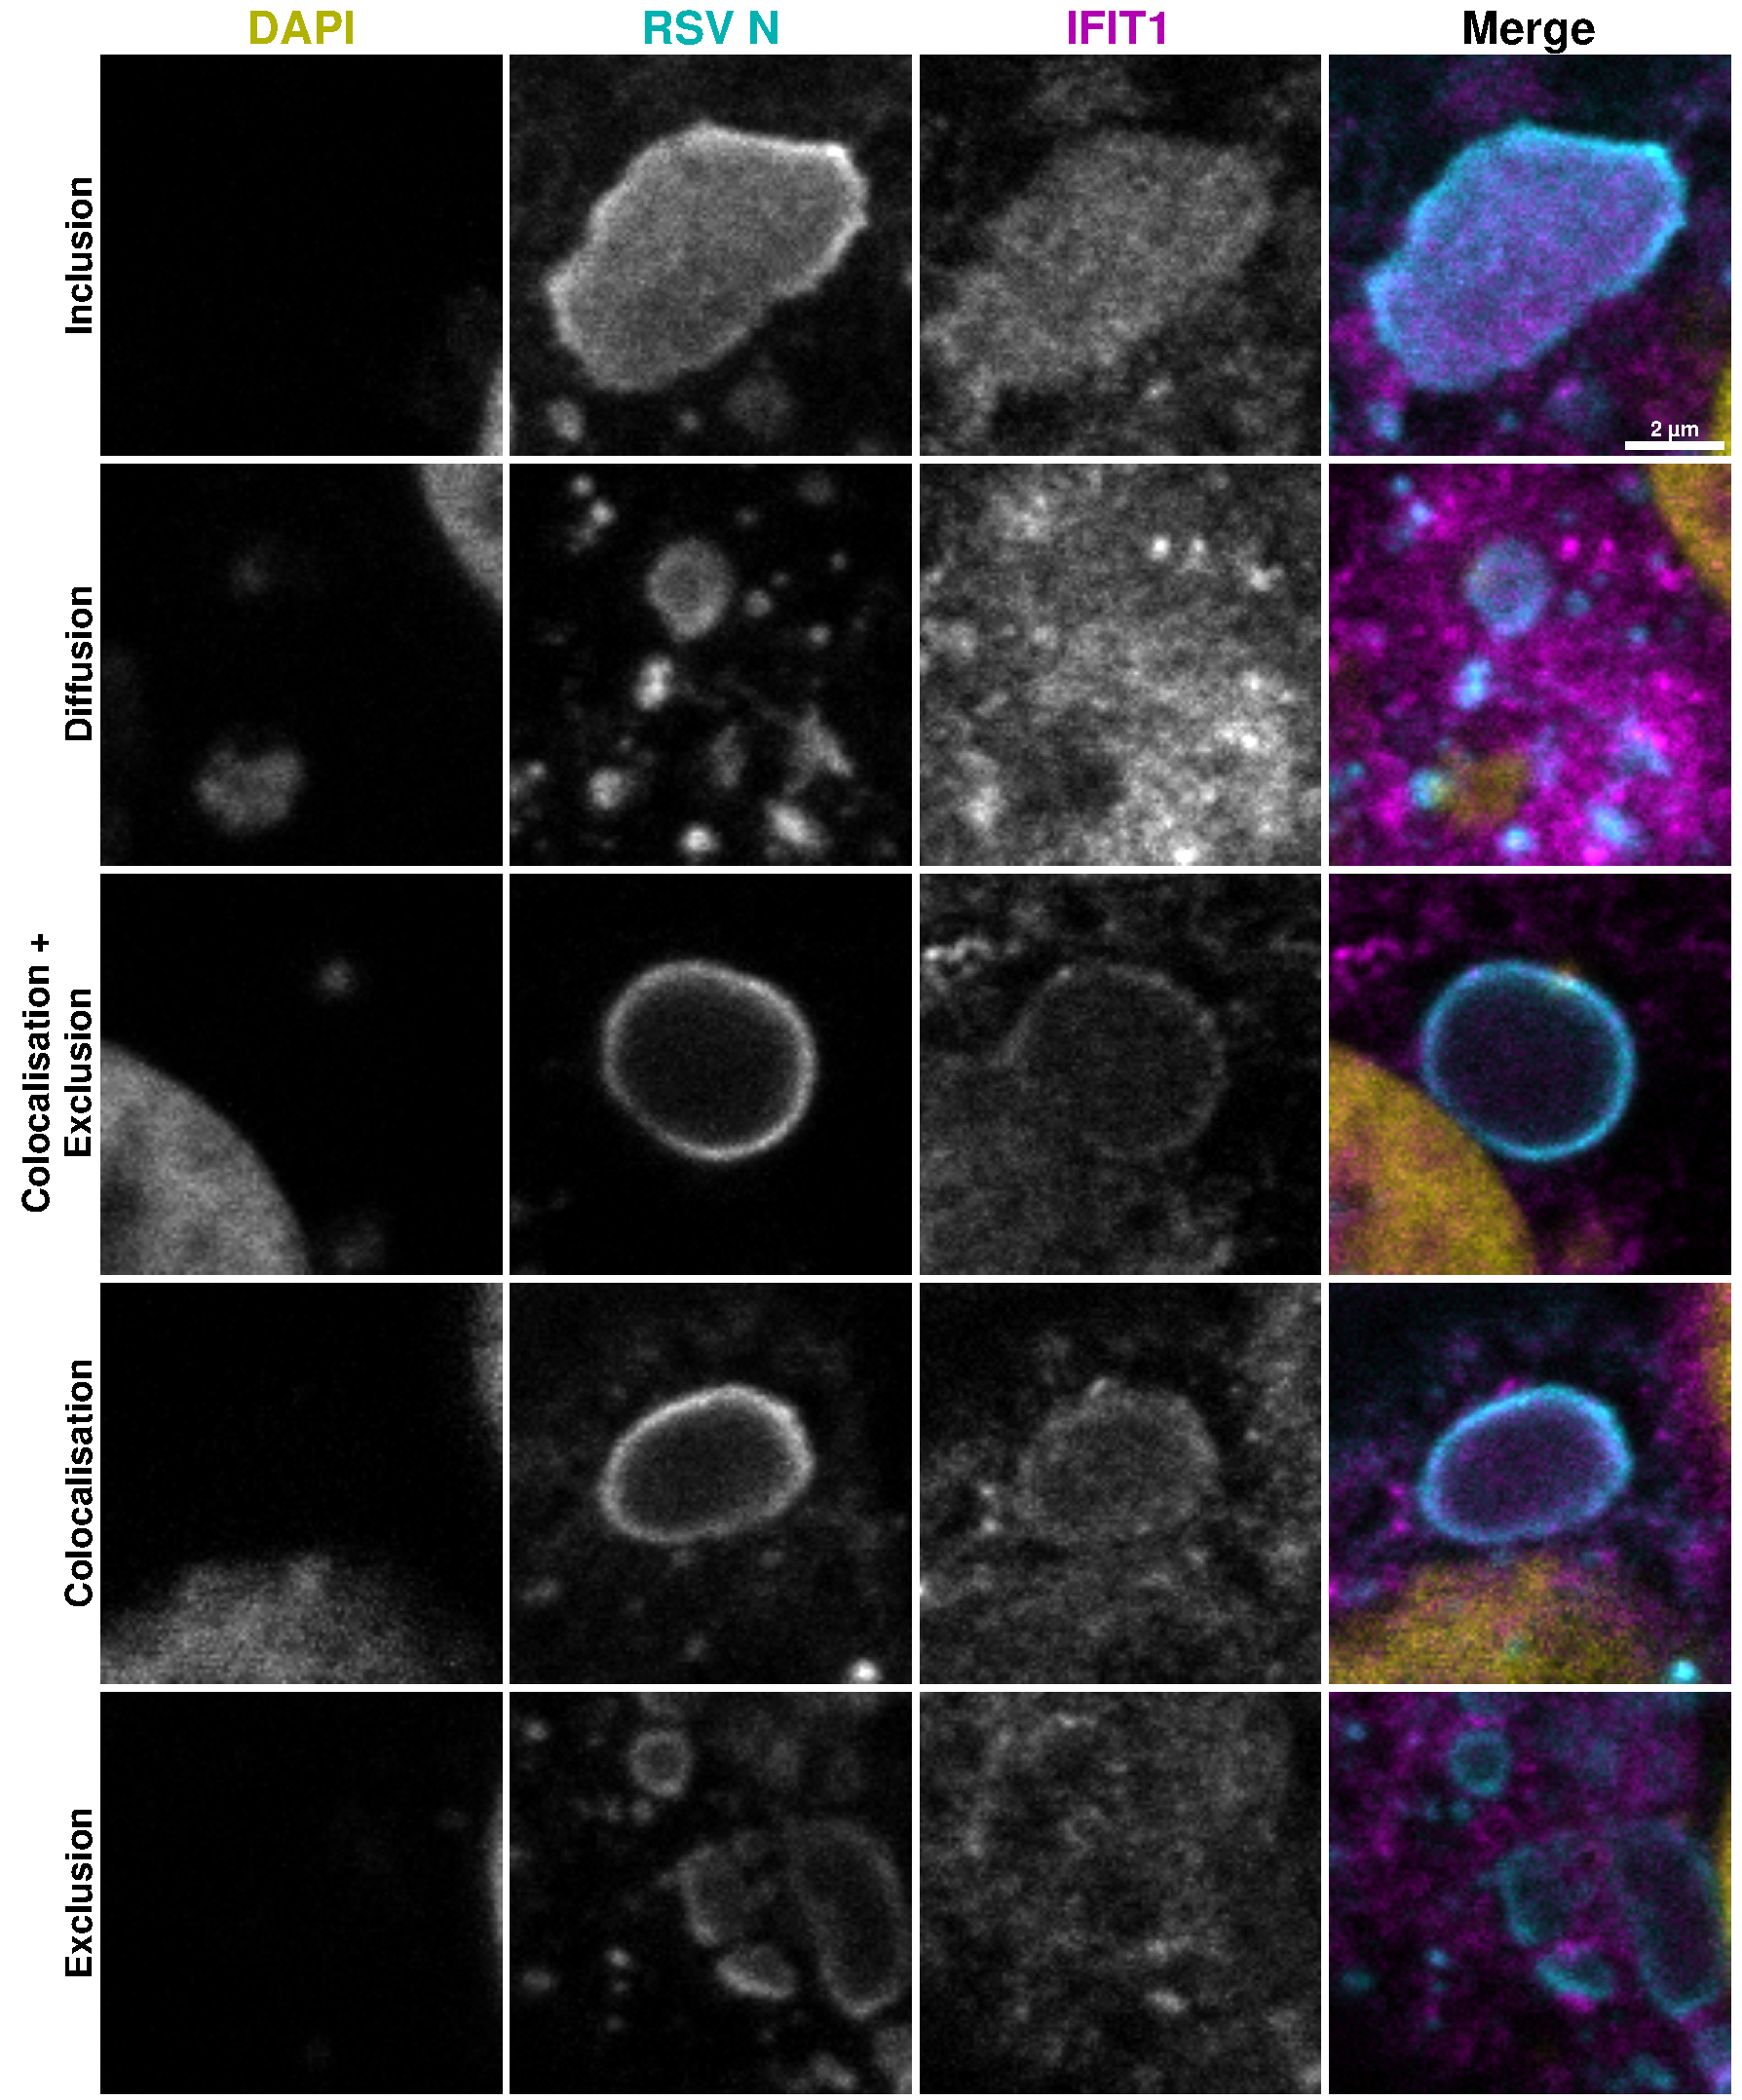
\includegraphics[width=1\linewidth]{08. Chapter 3/Figs/03. pIB/02. IFIT1/06. i1-vero-hnhp.pdf}
    \caption[Representative Images of Diverse Phenotypic Interactions of Monkey IFIT1 with Human Pseudo Inclusion Bodies (pIBs) in the VERO Cell Line.]{\textbf{Representative Images of Diverse Phenotypic Interactions of Monkey IFIT1 with Human Pseudo Inclusion Bodies (pIBs) in the VERO Cell Line.} Vero cells were transfected with hRSV N and P containing plasmids using TransIT-X2 and were fixed after 24 hours. Cellular nuclei were stained with DAPI (yellow), and cells were double-labeled with anti-RSV N (cyan) and anti-IFIT1 (magenta) antibodies. This figure showcases representative examples of relevant phenotypes in the interaction between monkey IFIT1 and hRSV pseudo inclusion bodies. These phenotypes are presented in descending order based on their percentage proportions. The scale bar indicates 2 \(\mu \mbox{m}\).}
    \label{fig:Representative Images of Diverse Phenotypic Interactions of Monkey IFIT1 with Human Pseudo Inclusion Bodies (pIBs) in the VERO Cell Line}
\end{figure}

43 38 8 5 5

2, 2, 9, 6, 1.1

In the context of bovine pIB structures, nascent monkey IFIT1 seems to colocalise with the edges of the structures (highlighted by the arrows). Consistent to human pIB data, nascent monkey IFIT1 is excluded from filamentous pIB network.

\begin{figure}
    \begin{subfigure}{0.495\textwidth}
        \caption{}
        \includegraphics[width=1\linewidth]{08. Chapter 3/Figs/03. pIB/02. IFIT1/07. bar_i1_vero_bnbp.pdf}  
    \end{subfigure}
    \begin{subfigure}{0.495\textwidth}
        \caption{}
        \includegraphics[width=1\linewidth]{08. Chapter 3/Figs/03. pIB/02. IFIT1/08. box_i1_vero_bnbp.pdf}
    \end{subfigure}
    \caption[Diverse Phenotypic Interactions of Monkey IFIT1 with Bovine Pseudo Inclusion Bodies (pIBs) in the VERO Cell Line.]{\textbf{Diverse Phenotypic Interactions of Monkey IFIT1 with Bovine Pseudo Inclusion Bodies (pIBs) in the VERO Cell Line.} Vero cells were transfected with bRSV N and P containing plasmids using TransIT-X2 and were fixed after 24 hours. Cells were labeled with anti-RSV N and anti-IFIT1 antibodies and imaged on confocal microscope. Panel (a) shows percentual proportions of observed phenotypes between bRSV pseudo inclusion bodies and monkey IFIT1 (14 observations), with the red dotted line denoting the 5\% threshold, marking phenotypes considered relevant above this limit. Panel (b) shows the IB area in \(\mu \mbox{m}^2\) per observed relevant phenotype.}
    \label{fig:Diverse Phenotypic Interactions of Monkey IFIT1 with Bovine Pseudo Inclusion Bodies (pIBs) in the VERO Cell Line}
\end{figure}

\begin{figure}
    \centering
    \includegraphics[width=1\linewidth]{08. Chapter 3/Figs/03. pIB/02. IFIT1/09. i1-vero-bnbp.pdf}
    \caption[Representative Images of Diverse Phenotypic Interactions of Monkey IFIT1 with Bovine Pseudo Inclusion Bodies (pIBs) in the VERO Cell Line.]{\textbf{Representative Images of Diverse Phenotypic Interactions of Monkey IFIT1 with Bovine Pseudo Inclusion Bodies (pIBs) in the VERO Cell Line.} Vero cells were transfected with bRSV N and P containing plasmids using TransIT-X2 and were fixed after 24 hours. Cellular nuclei were stained with DAPI (yellow), and cells were double-labeled with anti-RSV N (cyan) and anti-IFIT1 (magenta) antibodies. This figure showcases representative examples of relevant phenotypes in the interaction between monkey IFIT1 and bRSV pseudo inclusion bodies. These phenotypes are presented in descending order based on their percentage proportions. The scale bar indicates 2 \(\mu \mbox{m}\).}
    \label{fig:Representative Images of Diverse Phenotypic Interactions of Monkey IFIT1 with Bovine Pseudo Inclusion Bodies (pIBs) in the VERO Cell Line}
\end{figure}

56 44

1, 3

\subsubsection{IFIT2 Localisation in the Context of RSV pIBs}
%Single transfections
IFIT2 induction detected in hP and hP + hN conditions, suggesting that transfection of P induces IFIT2 expression (but this does not happen with IFIT1 or IFIT3 in the same cells).
About the different genomic regulation landscape… why does IFIT2 get induced but not other IFITs (within human genome which is well annotated)? 
Side note: No kinetochore microtubule staining (especially in first panel)

\begin{figure}
    \centering
    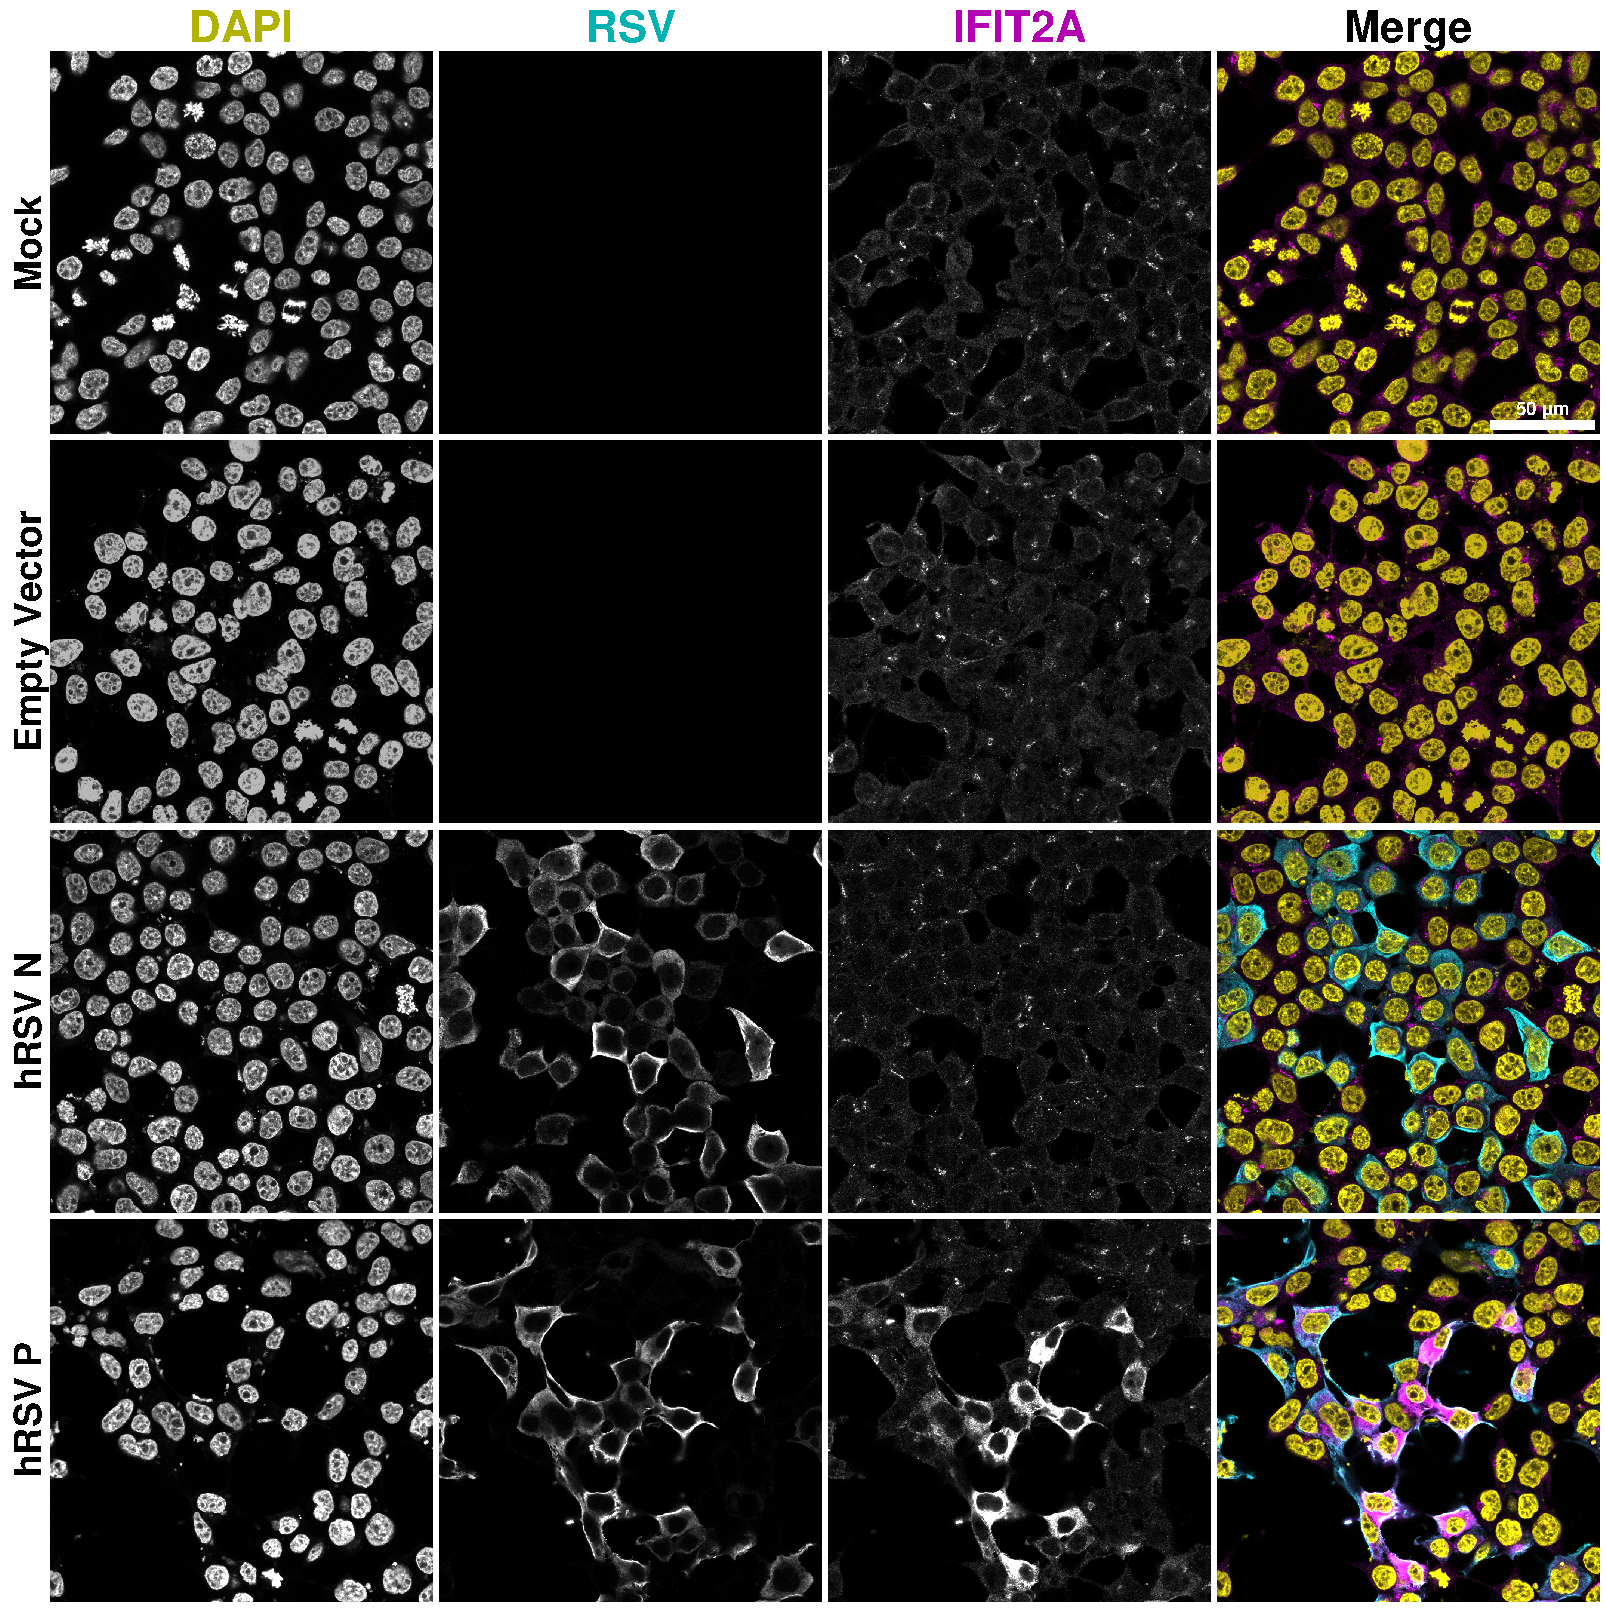
\includegraphics[width=1\linewidth]{08. Chapter 3/Figs/03. pIB/03. IFIT2/01. Single Transfection/01. 293t-ifit2a.pdf}
    \caption[IFIT2A Antibody Detects Increased IFIT2 Expression Following hRSV P Transfection.]{\textbf{IFIT2A Antibody Detects Increased IFIT2 Expression Following hRSV P Transfection.} 293T cells were either mock transfected, or single transfected with empty vector, hRSV N containing plasmid, or hRSV P containing plasmid using TransIT-X2 and were fixed after 24 hours. Cellular nuclei were stained with DAPI (yellow), and cells were double-labeled with either anti-RSV N (cyan), or anti-RSV P (cyan) and anti-IFIT2A (magenta) antibodies. The scale bar indicates 50 \(\mu \mbox{m}\).}
    \label{fig:IFIT2A Antibody Detects Increased IFIT2 Expression Following hRSV P Transfection}
\end{figure}

No detected IFIT2 induction in any of the conditions.
Side note: We can see kinetochore microtubule staining, especially in the first row.

\begin{figure}
    \centering
    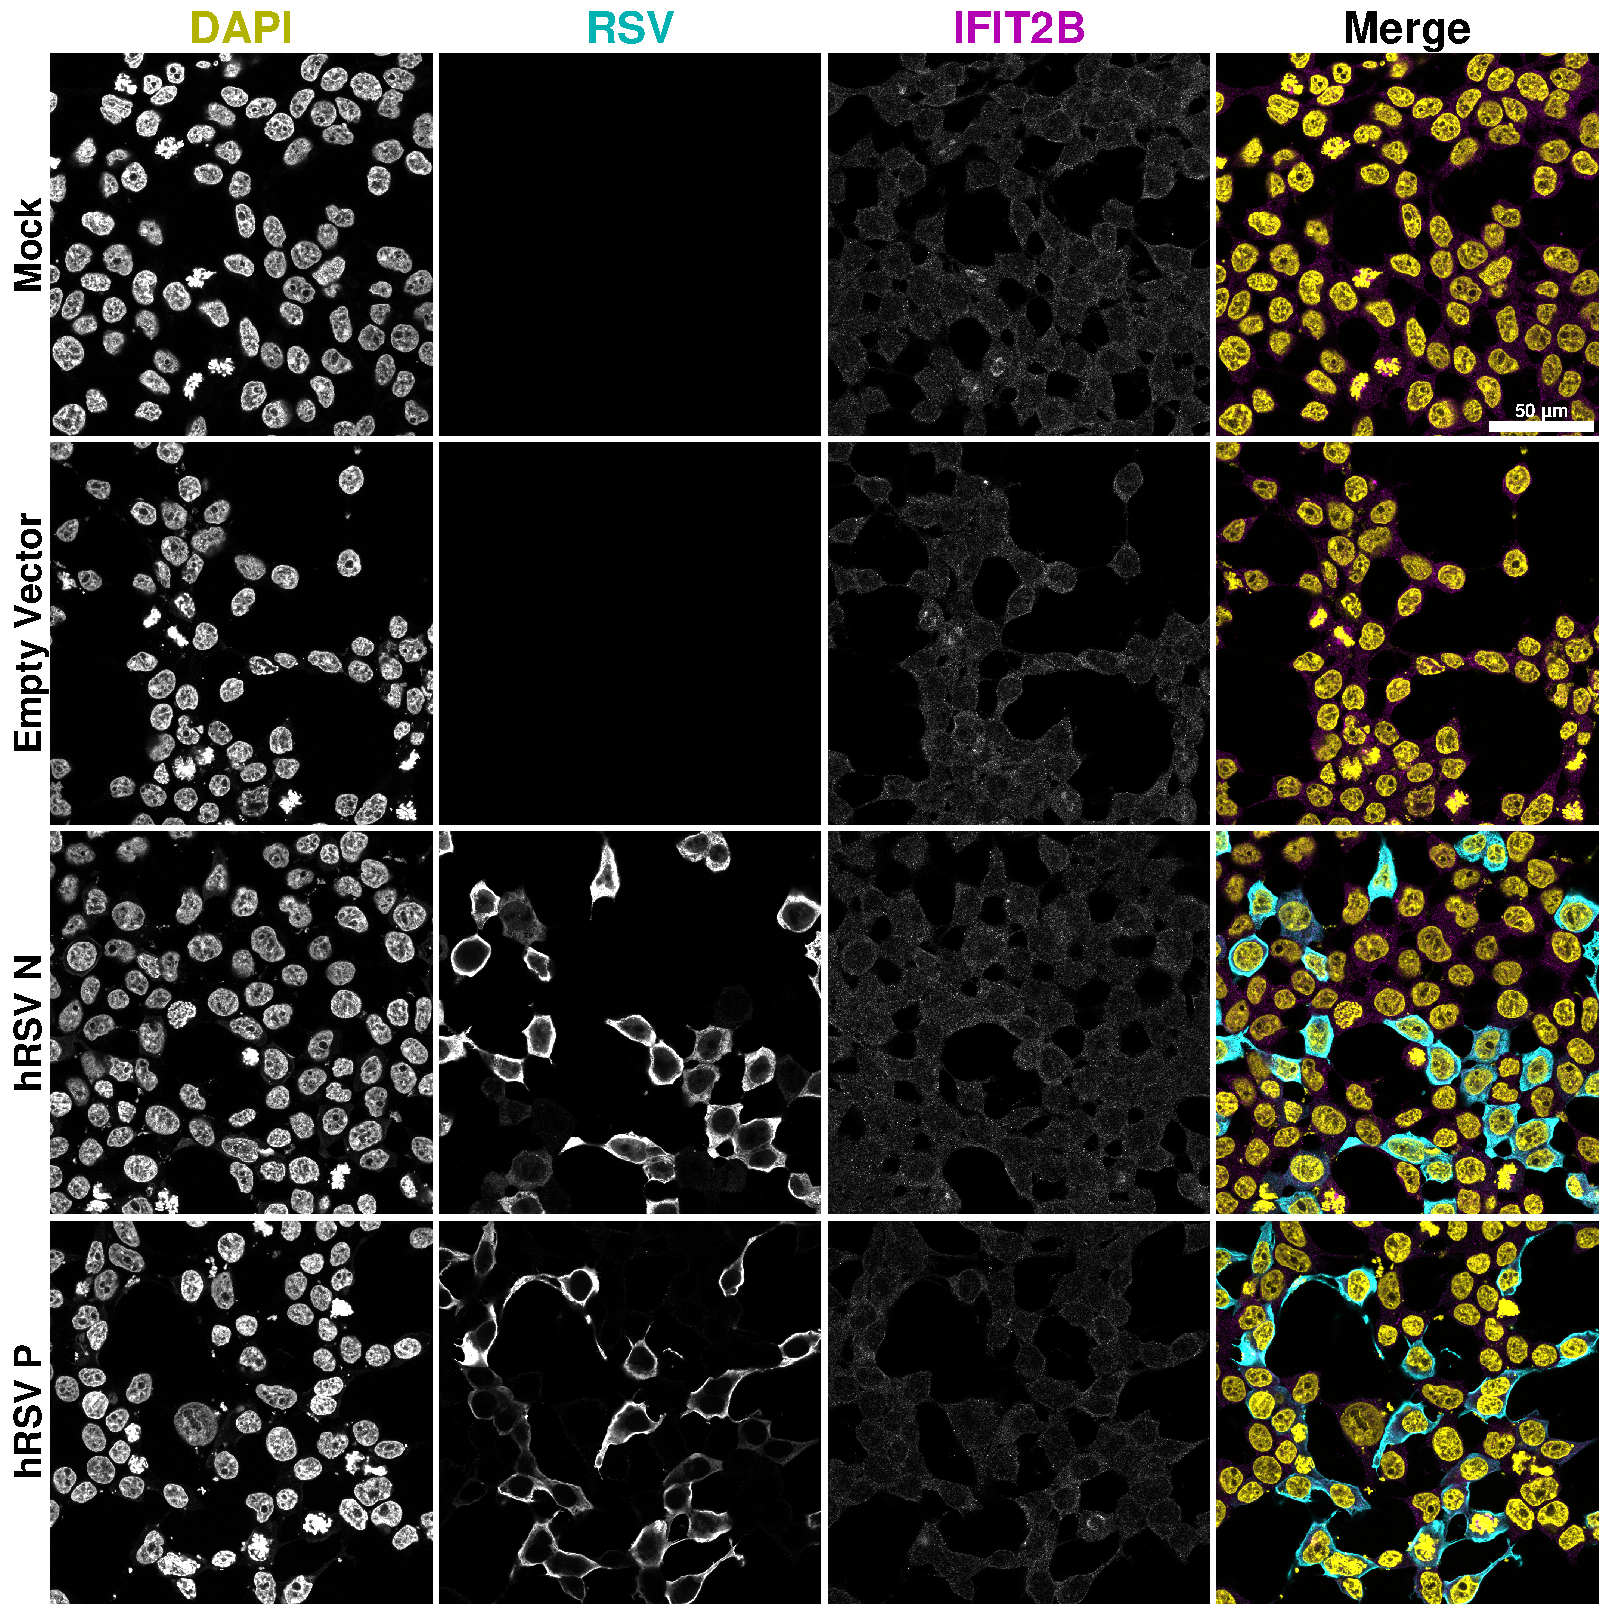
\includegraphics[width=1\linewidth]{08. Chapter 3/Figs/03. pIB/03. IFIT2/01. Single Transfection/02. 293t-ifit2b.pdf}
    \caption[IFIT2B Antibody Does Not Detect Increased IFIT2 Expression Following hRSV P Transfection.]{\textbf{IFIT2B Antibody Does Not Detect Increased IFIT2 Expression Following hRSV P Transfection.} 293T cells were either mock transfected, or single transfected with empty vector, hRSV N containing plasmid, or hRSV P containing plasmid using TransIT-X2 and were fixed after 24 hours. Cellular nuclei were stained with DAPI (yellow), and cells were double-labeled with either anti-RSV N (cyan), or anti-RSV P (cyan) and anti-IFIT2B (magenta) antibodies. The scale bar indicates 50 \(\mu \mbox{m}\).}
    \label{fig:IFIT2B Antibody Does Not Detect Increased IFIT2 Expression Following hRSV P Transfection}
\end{figure}

Nascent human IFIT2 strongly concentrates within the human RSV pseudo inclusion bodies.

\begin{figure}
    \begin{subfigure}{0.495\textwidth}
        \caption{}
        \includegraphics[width=1\linewidth]{08. Chapter 3/Figs/03. pIB/03. IFIT2/02. IFIT2A/01. bar_i2a_293t.pdf}
    \end{subfigure}
    \begin{subfigure}{0.495\textwidth}
        \caption{}
        \includegraphics[width=1\linewidth]{08. Chapter 3/Figs/03. pIB/03. IFIT2/02. IFIT2A/02. box_i2a_293t.pdf}
    \end{subfigure}
    \caption[Observed Phenotypes of Nascent Human IFIT2 in the Context of hRSV Pseudo Inclusion Bodies in 293T Cell Line, as Detected by IFIT2A Antibody.]{\textbf{Observed Phenotypes of Nascent Human IFIT2 in the Context of hRSV Pseudo Inclusion Bodies in 293T Cell Line, as Detected by IFIT2A Antibody.} 293T cells were transfected with hRSV N and P containing plasmids using TransIT-X2 and were fixed after 24 hours. Cells were labeled with anti-RSV N and anti-IFIT2A antibodies and imaged on confocal microscope. Panel (a) shows percentual proportions of observed phenotypes between hRSV pseudo inclusion bodies and human IFIT2 (81 observations), with the red dotted line denoting the 5\% threshold, marking phenotypes considered relevant above this limit. Panel (b) shows the IB area in \(\mu \mbox{m}^2\) per observed relevant phenotype.}
    \label{fig:Observed Phenotypes of Nascent Human IFIT2 in the Context of hRSV Pseudo Inclusion Bodies in 293T Cell Line, as Detected by IFIT2A Antibody}
\end{figure}

\begin{figure}
    \centering
    \includegraphics[width=1\linewidth]{08. Chapter 3/Figs/03. pIB/03. IFIT2/02. IFIT2A/03. i2a-293t-hnhp.pdf} 
    \caption[Representative Images of Observed Phenotypes of Nascent Human IFIT2 in the Context of hRSV Pseudo Inclusion Bodies in 293T Cell Line, as Detected by IFIT2A Antibody.]{\textbf{Representative Images of Observed Phenotypes of Nascent Human IFIT2 in the Context of hRSV Pseudo Inclusion Bodies in 293T Cell Line, as Detected by IFIT2A Antibody.} 293T cells were transfected with hRSV N and P containing plasmids using TransIT-X2 and were fixed after 24 hours. Cellular nuclei were stained with DAPI (yellow), and cells were double-labeled with anti-RSV N (cyan) and anti-IFIT2A (magenta) antibodies. This figure showcases representative examples of relevant phenotypes in the interaction between human IFIT2 and hRSV pseudo inclusion bodies. These phenotypes are presented in descending order based on their percentage proportions. The scale bar indicates 2 \(\mu \mbox{m}\).}
    \label{fig:Representative Images of Observed Phenotypes of Nascent Human IFIT2 in the Context of hRSV Pseudo Inclusion Bodies in 293T Cell Line, as Detected by IFIT2A Antibody}
\end{figure}

99
2

Endogenous monkey IFIT2 colocalises with the pIB structure (probably like an inclusion), as well as with the pIB filamentous network.

\begin{figure}
    \begin{subfigure}{0.495\textwidth}
        \caption{}
        \includegraphics[width=1\linewidth]{08. Chapter 3/Figs/03. pIB/03. IFIT2/02. IFIT2A/04. bar_i2a_vero_hnhp.pdf} 
    \end{subfigure}
    \begin{subfigure}{0.495\textwidth}
        \caption{}
        \includegraphics[width=1\linewidth]{08. Chapter 3/Figs/03. pIB/03. IFIT2/02. IFIT2A/05. box_i2a_vero_hnhp.pdf}
    \end{subfigure}
    \caption[Observed Phenotypes of Nascent Monkey IFIT2 in the Context of hRSV Pseudo Inclusion Bodies in VERO Cell Line, as Detected by IFIT2A Antibody.]{\textbf{Observed Phenotypes of Nascent Monkey IFIT2 in the Context of hRSV Pseudo Inclusion Bodies in VERO Cell Line, as Detected by IFIT2A Antibody.} Vero cells were transfected with hRSV N and P containing plasmids using TransIT-X2 and were fixed after 24 hours. Cells were labeled with anti-RSV N and anti-IFIT2A antibodies and imaged on confocal microscope. Panel (a) shows percentual proportions of observed phenotypes between hRSV pseudo inclusion bodies and monkey IFIT2 (48 observations), with the red dotted line denoting the 5\% threshold, marking phenotypes considered relevant above this limit. Panel (b) shows the IB area in \(\mu \mbox{m}^2\) per observed relevant phenotype.}
    \label{fig:Observed Phenotypes of Nascent Monkey IFIT2 in the Context of hRSV Pseudo Inclusion Bodies in VERO Cell Line, as Detected by IFIT2A Antibody}
\end{figure}

\begin{figure}
    \centering
    \includegraphics[width=1\linewidth]{08. Chapter 3/Figs/03. pIB/03. IFIT2/02. IFIT2A/06. i2a-vero-hnhp.pdf}  
    \caption[Representative Images of Observed Phenotypes of Nascent Human IFIT2 in the Context of hRSV Pseudo Inclusion Bodies in VERO Cell Line, as Detected by IFIT2A Antibody.]{\textbf{Representative Images of Observed Phenotypes of Nascent Human IFIT2 in the Context of hRSV Pseudo Inclusion Bodies in VERO Cell Line, as Detected by IFIT2A Antibody.} Vero cells were transfected with hRSV N and P containing plasmids using TransIT-X2 and were fixed after 24 hours. Cellular nuclei were stained with DAPI (yellow), and cells were double-labeled with anti-RSV N (cyan) and anti-IFIT2A (magenta) antibodies. This figure showcases representative examples of relevant phenotypes in the interaction between monkey IFIT2 and hRSV pseudo inclusion bodies. These phenotypes are presented in descending order based on their percentage proportions. The scale bar indicates 2 \(\mu \mbox{m}\).}
    \label{fig:Representative Images of Observed Phenotypes of Nascent Human IFIT2 in the Context of hRSV Pseudo Inclusion Bodies in VERO Cell Line, as Detected by IFIT2A Antibody}
\end{figure}

100
1.2

\begin{figure}
    \begin{subfigure}{0.495\textwidth}
        \caption{}
        \includegraphics[width=1\linewidth]{08. Chapter 3/Figs/03. pIB/03. IFIT2/02. IFIT2A/07. bar_i2a_vero_bnbp.pdf} 
    \end{subfigure}
    \begin{subfigure}{0.495\textwidth}
        \caption{}
        \includegraphics[width=1\linewidth]{08. Chapter 3/Figs/03. pIB/03. IFIT2/02. IFIT2A/08. box_i2a_vero_bnbp.pdf}
    \end{subfigure}
    \caption[Observed Phenotypes of Nascent Monkey IFIT2 in the Context of bRSV Pseudo Inclusion Bodies in VERO Cell Line, as Detected by IFIT2A Antibody.]{\textbf{Observed Phenotypes of Nascent Monkey IFIT2 in the Context of bRSV Pseudo Inclusion Bodies in VERO Cell Line, as Detected by IFIT2A Antibody.} Vero cells were transfected with bRSV N and P containing plasmids using TransIT-X2 and were fixed after 24 hours. Cells were labeled with anti-RSV N and anti-IFIT2A antibodies and imaged on confocal microscope. Panel (a) shows percentual proportions of observed phenotypes between bRSV pseudo inclusion bodies and monkey IFIT2 (38 observations), with the red dotted line denoting the 5\% threshold, marking phenotypes considered relevant above this limit. Panel (b) shows the IB area in \(\mu \mbox{m}^2\) per observed relevant phenotype.}
    \label{fig:Observed Phenotypes of Nascent Monkey IFIT2 in the Context of bRSV Pseudo Inclusion Bodies in VERO Cell Line, as Detected by IFIT2A Antibody}
\end{figure}

\begin{figure}
    \centering
    \includegraphics[width=1\linewidth]{08. Chapter 3/Figs/03. pIB/03. IFIT2/02. IFIT2A/09. i2a-vero-bnbp.pdf} 
    \caption[Representative Images of Observed Phenotypes of Nascent Human IFIT2 in the Context of bRSV Pseudo Inclusion Bodies in VERO Cell Line, as Detected by IFIT2A Antibody.]{\textbf{Representative Images of Observed Phenotypes of Nascent Human IFIT2 in the Context of bRSV Pseudo Inclusion Bodies in VERO Cell Line, as Detected by IFIT2A Antibody.} Vero cells were transfected with bRSV N and P containing plasmids using TransIT-X2 and were fixed after 24 hours. Cellular nuclei were stained with DAPI (yellow), and cells were double-labeled with anti-RSV N (cyan) and anti-IFIT2A (magenta) antibodies. This figure showcases representative examples of relevant phenotypes in the interaction between monkey IFIT2 and bRSV pseudo inclusion bodies. These phenotypes are presented in descending order based on their percentage proportions. The scale bar indicates 2 \(\mu \mbox{m}\).}
    \label{fig:Representative Images of Observed Phenotypes of Nascent Human IFIT2 in the Context of bRSV Pseudo Inclusion Bodies in VERO Cell Line, as Detected by IFIT2A Antibody}
\end{figure}

100
1.8

Nascent monkey IFIT2 is completely excluded from the human RSV pseudo-IBs and the pIB filamentous network.

\begin{figure}
    \begin{subfigure}{0.495\textwidth}
        \caption{}
        \includegraphics[width=1\linewidth]{08. Chapter 3/Figs/03. pIB/03. IFIT2/03. IFIT2B/01. bar_i2b_293t.pdf} 
    \end{subfigure}
    \begin{subfigure}{0.495\textwidth}
        \caption{}
        \includegraphics[width=1\linewidth]{08. Chapter 3/Figs/03. pIB/03. IFIT2/03. IFIT2B/02. box_i2b_293t.pdf}
    \end{subfigure}
    \caption[Observed Phenotypes of Nascent Human IFIT2 in the Context of hRSV Pseudo Inclusion Bodies in 293T Cell Line, as Detected by IFIT2B Antibody.]{\textbf{Observed Phenotypes of Nascent Human IFIT2 in the Context of hRSV Pseudo Inclusion Bodies in 293T Cell Line, as Detected by IFIT2B Antibody.} 293T cells were transfected with hRSV N and P containing plasmids using TransIT-X2 and were fixed after 24 hours. Cells were labeled with anti-RSV N and anti-IFIT2B antibodies and imaged on confocal microscope. Panel (a) shows percentual proportions of observed phenotypes between hRSV pseudo inclusion bodies and human IFIT2 (6 observations), with the red dotted line denoting the 5\% threshold, marking phenotypes considered relevant above this limit. Panel (b) shows the IB area in \(\mu \mbox{m}^2\) per observed relevant phenotype.}
    \label{fig:Observed Phenotypes of Nascent Human IFIT2 in the Context of hRSV Pseudo Inclusion Bodies in 293T Cell Line, as Detected by IFIT2B Antibody}
\end{figure}

\begin{figure}
    \centering
    \includegraphics[width=1\linewidth]{08. Chapter 3/Figs/03. pIB/03. IFIT2/03. IFIT2B/03. i2b-293t-hnhp.pdf} 
    \caption[Representative Images of Observed Phenotypes of Nascent Human IFIT2 in the Context of hRSV Pseudo Inclusion Bodies in 293T Cell Line, as Detected by IFIT2B Antibody.]{\textbf{Representative Images of Observed Phenotypes of Nascent Human IFIT2 in the Context of hRSV Pseudo Inclusion Bodies in 293T Cell Line, as Detected by IFIT2B Antibody.} 293T cells were transfected with hRSV N and P containing plasmids using TransIT-X2 and were fixed after 24 hours. Cellular nuclei were stained with DAPI (yellow), and cells were double-labeled with anti-RSV N (cyan) and anti-IFIT2B (magenta) antibodies. This figure showcases representative examples of relevant phenotypes in the interaction between human IFIT2 and hRSV pseudo inclusion bodies. These phenotypes are presented in descending order based on their percentage proportions. The scale bar indicates 2 \(\mu \mbox{m}\).}
    \label{fig:Representative Images of Observed Phenotypes of Nascent Human IFIT2 in the Context of hRSV Pseudo Inclusion Bodies in 293T Cell Line, as Detected by IFIT2B Antibody}
\end{figure}

100
4

\begin{figure}
    \begin{subfigure}{0.495\textwidth}
        \caption{}
        \includegraphics[width=1\linewidth]{08. Chapter 3/Figs/03. pIB/03. IFIT2/03. IFIT2B/04. bar_i2b_vero_hnhp.pdf} 
    \end{subfigure}
    \begin{subfigure}{0.495\textwidth}
        \caption{}
        \includegraphics[width=1\linewidth]{08. Chapter 3/Figs/03. pIB/03. IFIT2/03. IFIT2B/05. box_i2b_vero_hnhp.pdf}
    \end{subfigure}
    \caption[Observed Phenotypes of Nascent Monkey IFIT2 in the Context of hRSV Pseudo Inclusion Bodies in VERO Cell Line, as Detected by IFIT2B Antibody.]{\textbf{Observed Phenotypes of Nascent Monkey IFIT2 in the Context of hRSV Pseudo Inclusion Bodies in VERO Cell Line, as Detected by IFIT2B Antibody.} Vero cells were transfected with hRSV N and P containing plasmids using TransIT-X2 and were fixed after 24 hours. Cells were labeled with anti-RSV N and anti-IFIT2B antibodies and imaged on confocal microscope. Panel (a) shows percentual proportions of observed phenotypes between hRSV pseudo inclusion bodies and monkey IFIT2 (76 observations), with the red dotted line denoting the 5\% threshold, marking phenotypes considered relevant above this limit. Panel (b) shows the IB area in \(\mu \mbox{m}^2\) per observed relevant phenotype.}
    \label{fig:Observed Phenotypes of Nascent Monkey IFIT2 in the Context of hRSV Pseudo Inclusion Bodies in VERO Cell Line, as Detected by IFIT2B Antibody}
\end{figure}

\begin{figure}
    \centering
    \includegraphics[width=1\linewidth]{08. Chapter 3/Figs/03. pIB/03. IFIT2/03. IFIT2B/06. i2b-vero-hnhp.pdf} 
    \caption[Representative Images of Observed Phenotypes of Nascent Human IFIT2 in the Context of hRSV Pseudo Inclusion Bodies in VERO Cell Line, as Detected by IFIT2B Antibody.]{\textbf{Representative Images of Observed Phenotypes of Nascent Human IFIT2 in the Context of hRSV Pseudo Inclusion Bodies in VERO Cell Line, as Detected by IFIT2B Antibody.} Vero cells were transfected with hRSV N and P containing plasmids using TransIT-X2 and were fixed after 24 hours. Cellular nuclei were stained with DAPI (yellow), and cells were double-labeled with anti-RSV N (cyan) and anti-IFIT2B (magenta) antibodies. This figure showcases representative examples of relevant phenotypes in the interaction between monkey IFIT2 and hRSV pseudo inclusion bodies. These phenotypes are presented in descending order based on their percentage proportions. The scale bar indicates 2 \(\mu \mbox{m}\).}
    \label{fig:Representative Images of Observed Phenotypes of Nascent Human IFIT2 in the Context of hRSV Pseudo Inclusion Bodies in VERO Cell Line, as Detected by IFIT2B Antibody}
\end{figure}

91 9
2 0.63

% summary
Both endogenous human and monkey IFIT2 forms inclusions inside human RSV pseudo-IBs. Monkey IFIT2 also colocalises to the pIB filamentous network (this structure was not observed in the human experiment). The identical staining can be observed in monkey cells with overexpressed human IFIT2-FLAG.

Endogenous monkey IFIT2 is excluded from human pIB and the pIB associated filamentous network. Overexpressed human IFIT2-FLAG is detected by the antibody and shows inclusions inside the human pIB structures, which is consistent to data from IFIT2A staining and FLAG staining of IFIT2-FLAG overexpressed samples. Interestingly, IFIT2B antibody shows exclusion from the pIB filamentous network, which was colocalised by IFIT2A and FLAG antibodies.

\paragraph{Exogenous IFIT2-FLAG Localisation in the Context of RSV pIBs}
Monkey cells transfected with human RSV N and P, along with human IFIT2-FLAG show concentration within the pIB structures as well as the pIB filamentous network. In this experiment we are detecting both human and monkey IFIT2, however we can see a huge difference in IFIT2 expression between some cells (bottom panel; cells in the periphery of the picture), suggesting that what we are mainly detecting is the overexpressed human IFIT2-FLAG.

\begin{figure}
    \begin{subfigure}{0.495\textwidth}
        \caption{}
        \includegraphics[width=1\linewidth]{08. Chapter 3/Figs/03. pIB/03. IFIT2/04. IFIT2-FLAG/01. IFIT2A/01. bar_i2a_hnhp.pdf} 
    \end{subfigure}
    \begin{subfigure}{0.495\textwidth}
        \caption{}
        \includegraphics[width=1\linewidth]{08. Chapter 3/Figs/03. pIB/03. IFIT2/04. IFIT2-FLAG/01. IFIT2A/02. box_i2a_hnhp.pdf}
    \end{subfigure}
    \caption[Observed Phenotypes of Exogenous Human IFIT2 in the Context of hRSV Pseudo Inclusion Bodies in VERO Cell Line, as Detected by IFIT2A Antibody.]{\textbf{Observed Phenotypes of Exogenous Human IFIT2 in the Context of hRSV Pseudo Inclusion Bodies in VERO Cell Line, as Detected by IFIT2A Antibody.} Vero cells were transfected with hRSV N and P, along with human IFIT2-FLAG containing plasmids using TransIT-X2 and were fixed after 24 hours. Cells were labeled with anti-RSV N and anti-IFIT2A antibodies and imaged on confocal microscope. Panel (a) shows percentual proportions of observed phenotypes between hRSV pseudo inclusion bodies and exogenous human IFIT2 (56 observations), with the red dotted line denoting the 5\% threshold, marking phenotypes considered relevant above this limit. Panel (b) shows the IB area in \(\mu \mbox{m}^2\) per observed relevant phenotype.}
    \label{fig:Observed Phenotypes of Exogenous Human IFIT2 in the Context of hRSV Pseudo Inclusion Bodies in VERO Cell Line, as Detected by IFIT2A Antibody}
\end{figure}

\begin{figure}
    \centering
    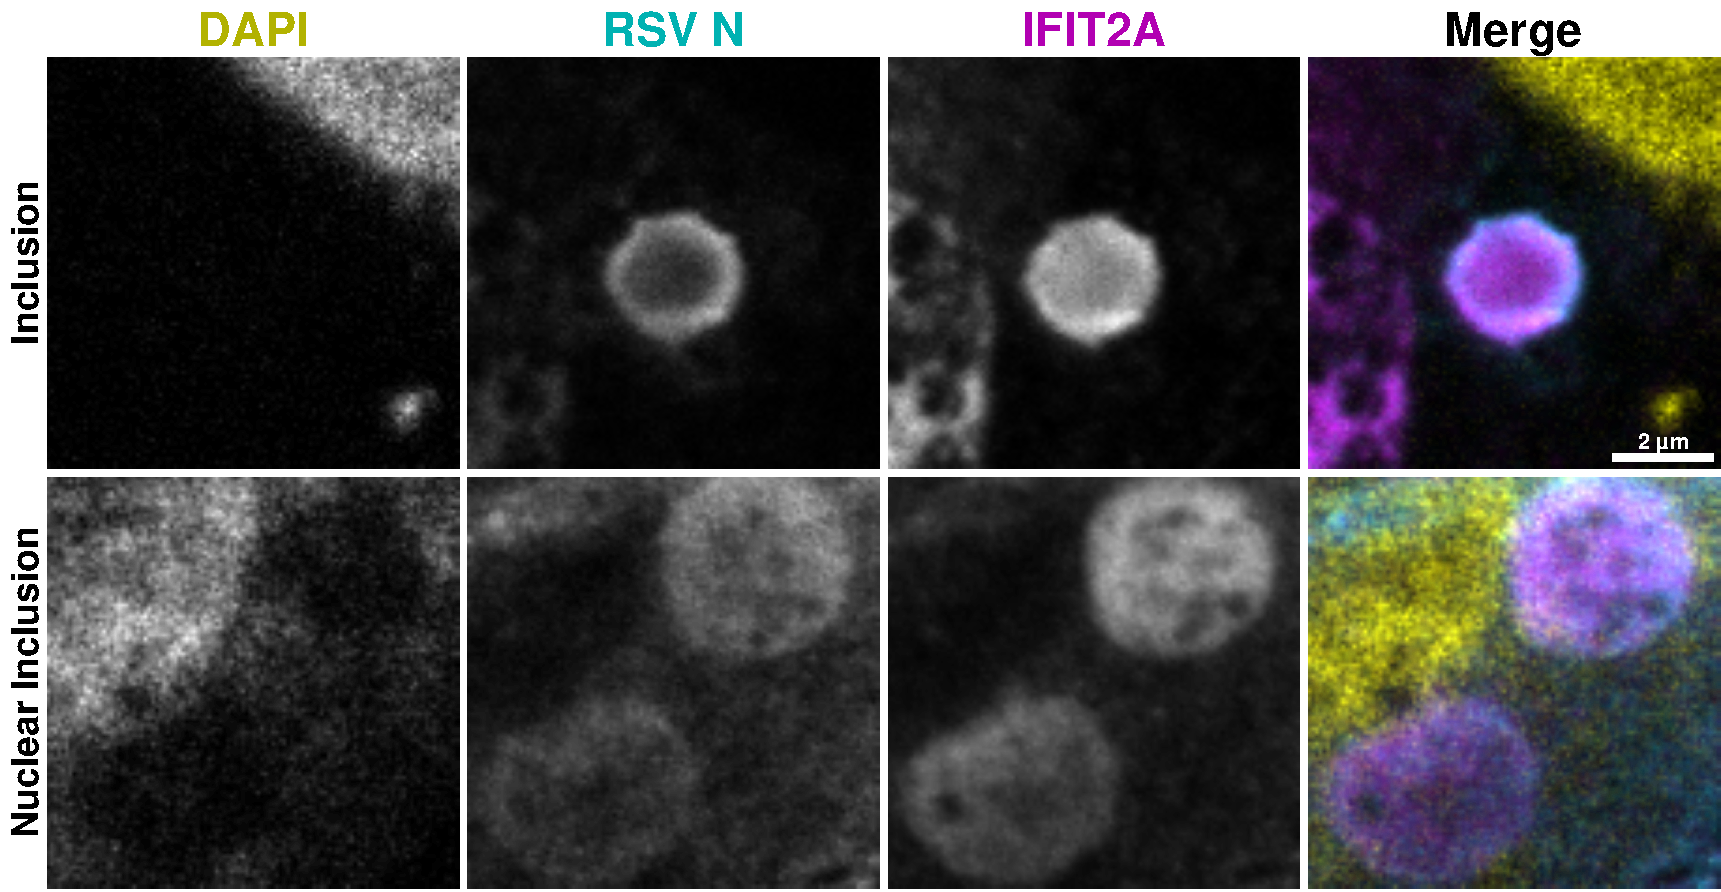
\includegraphics[width=1\linewidth]{08. Chapter 3/Figs/03. pIB/03. IFIT2/04. IFIT2-FLAG/01. IFIT2A/03. i2a-hi2f-hnhp.pdf}
    \caption[Representative Images of Observed Phenotypes of Exogenous Human IFIT2 in the Context of hRSV Pseudo Inclusion Bodies in VERO Cell Line, as Detected by IFIT2A Antibody.]{\textbf{Representative Images of Observed Phenotypes of Exogenous Human IFIT2 in the Context of hRSV Pseudo Inclusion Bodies in VERO Cell Line, as Detected by IFIT2A Antibody.} Vero cells were transfected with hRSV N and P, along with human IFIT2-FLAG containing plasmids using TransIT-X2 and were fixed after 24 hours. Cellular nuclei were stained with DAPI (yellow), and cells were double-labeled with anti-RSV N (cyan) and anti-IFIT2A (magenta) antibodies. This figure showcases representative examples of relevant phenotypes in the interaction between exogenous human IFIT2 and hRSV pseudo inclusion bodies. These phenotypes are presented in descending order based on their percentage proportions. The scale bar indicates 2 \(\mu \mbox{m}\).}
    \label{fig:Representative Images of Observed Phenotypes of Exogenous Human IFIT2 in the Context of hRSV Pseudo Inclusion Bodies in VERO Cell Line, as Detected by IFIT2A Antibody}
\end{figure}

100
0.9

Monkey cells transfected with human RSV N and P, along with human IFIT2-FLAG show concentration within the pIB structures but show exclusion from the pIB filamentous network (or partial colocalsiation?). This suggest that the IFIT2B antibody can indeed detect IFIT2 but the overexpressed IFIT2 observed between the inclusion and the one interacting with the filamentous network is somehow different (epitope masking?).

\begin{figure}
    \begin{subfigure}{0.495\textwidth}
        \caption{}
        \includegraphics[width=1\linewidth]{08. Chapter 3/Figs/03. pIB/03. IFIT2/04. IFIT2-FLAG/02. IFIT2B/01. bar_i2b_hnhp.pdf}
    \end{subfigure}
    \begin{subfigure}{0.495\textwidth}
        \caption{}
        \includegraphics[width=1\linewidth]{08. Chapter 3/Figs/03. pIB/03. IFIT2/04. IFIT2-FLAG/02. IFIT2B/02. box_i2a_hnhp.pdf}
    \end{subfigure}
    \caption[Observed Phenotypes of Exogenous Human IFIT2 in the Context of hRSV Pseudo Inclusion Bodies in VERO Cell Line, as Detected by IFIT2B Antibody.]{\textbf{Observed Phenotypes of Exogenous Human IFIT2 in the Context of hRSV Pseudo Inclusion Bodies in VERO Cell Line, as Detected by IFIT2B Antibody.} Vero cells were transfected with hRSV N and P, along with human IFIT2-FLAG containing plasmids using TransIT-X2 and were fixed after 24 hours. Cells were labeled with anti-RSV N and anti-IFIT2B antibodies and imaged on confocal microscope. Panel (a) shows percentual proportions of observed phenotypes between hRSV pseudo inclusion bodies and exogenous human IFIT2 (44 observations), with the red dotted line denoting the 5\% threshold, marking phenotypes considered relevant above this limit. Panel (b) shows the IB area in \(\mu \mbox{m}^2\) per observed relevant phenotype.}
    \label{fig:Observed Phenotypes of Exogenous Human IFIT2 in the Context of hRSV Pseudo Inclusion Bodies in VERO Cell Line, as Detected by IFIT2B Antibody}
\end{figure}

\begin{figure}
    \centering
    \includegraphics[width=1\linewidth]{08. Chapter 3/Figs/03. pIB/03. IFIT2/04. IFIT2-FLAG/02. IFIT2B/03. i2b-hi2f-hnhp.pdf}
    \caption[Representative Images of Observed Phenotypes of Exogenous Human IFIT2 in the Context of hRSV Pseudo Inclusion Bodies in VERO Cell Line, as Detected by IFIT2B Antibody.]{\textbf{Representative Images of Observed Phenotypes of Exogenous Human IFIT2 in the Context of hRSV Pseudo Inclusion Bodies in VERO Cell Line, as Detected by IFIT2B Antibody.} Vero cells were transfected with hRSV N and P, along with human IFIT2-FLAG containing plasmids using TransIT-X2 and were fixed after 24 hours. Cellular nuclei were stained with DAPI (yellow), and cells were double-labeled with anti-RSV N (cyan) and anti-IFIT2B (magenta) antibodies. This figure showcases representative examples of relevant phenotypes in the interaction between exogenous human IFIT2 and hRSV pseudo inclusion bodies. These phenotypes are presented in descending order based on their percentage proportions. The scale bar indicates 2 \(\mu \mbox{m}\).}
    \label{fig:Representative Images of Observed Phenotypes of Exogenous Human IFIT2 in the Context of hRSV Pseudo Inclusion Bodies in VERO Cell Line, as Detected by IFIT2B Antibody}
\end{figure}

50 47
3.2 0.4

Exogenously expressed human IFIT2 colocalises with the pIB associated filamentous net (top panel). It also forms inclusion inside the human pIB structures. This data is consistent with what we observed with IFIT2A antibody. IFIT2 also seems to occasionally form aggregates/spots (highlighted by arrows). These could be functional or just aggregates caused by overexpression, we do not know.

\begin{figure}
    \begin{subfigure}{0.495\textwidth}
        \caption{}
        \includegraphics[width=1\linewidth]{08. Chapter 3/Figs/03. pIB/03. IFIT2/04. IFIT2-FLAG/03. FLAG/01. bar_hi2f_hnhp.pdf}
    \end{subfigure}
    \begin{subfigure}{0.495\textwidth}
        \caption{}
        \includegraphics[width=1\linewidth]{08. Chapter 3/Figs/03. pIB/03. IFIT2/04. IFIT2-FLAG/03. FLAG/02. box_hi2f_hnhp.pdf}
    \end{subfigure}
    \caption[Observed Phenotypes of Exogenous Human IFIT2 in the Context of hRSV Pseudo Inclusion Bodies in VERO Cell Line, as Detected by FLAG Antibody.]{\textbf{Observed Phenotypes of Exogenous Human IFIT2 in the Context of hRSV Pseudo Inclusion Bodies in VERO Cell Line, as Detected by FLAG Antibody.} Vero cells were transfected with hRSV N and P, along with human IFIT2-FLAG containing plasmids using TransIT-X2 and were fixed after 24 hours. Cells were labeled with anti-RSV N and anti-FLAG antibodies and imaged on confocal microscope. Panel (a) shows percentual proportions of observed phenotypes between hRSV pseudo inclusion bodies and exogenous human IFIT2 (116 observations), with the red dotted line denoting the 5\% threshold, marking phenotypes considered relevant above this limit. Panel (b) shows the IB area in \(\mu \mbox{m}^2\) per observed relevant phenotype.}
    \label{fig:Observed Phenotypes of Exogenous Human IFIT2 in the Context of hRSV Pseudo Inclusion Bodies in VERO Cell Line, as Detected by FLAG Antibody}
\end{figure}

\begin{figure}
    \centering
    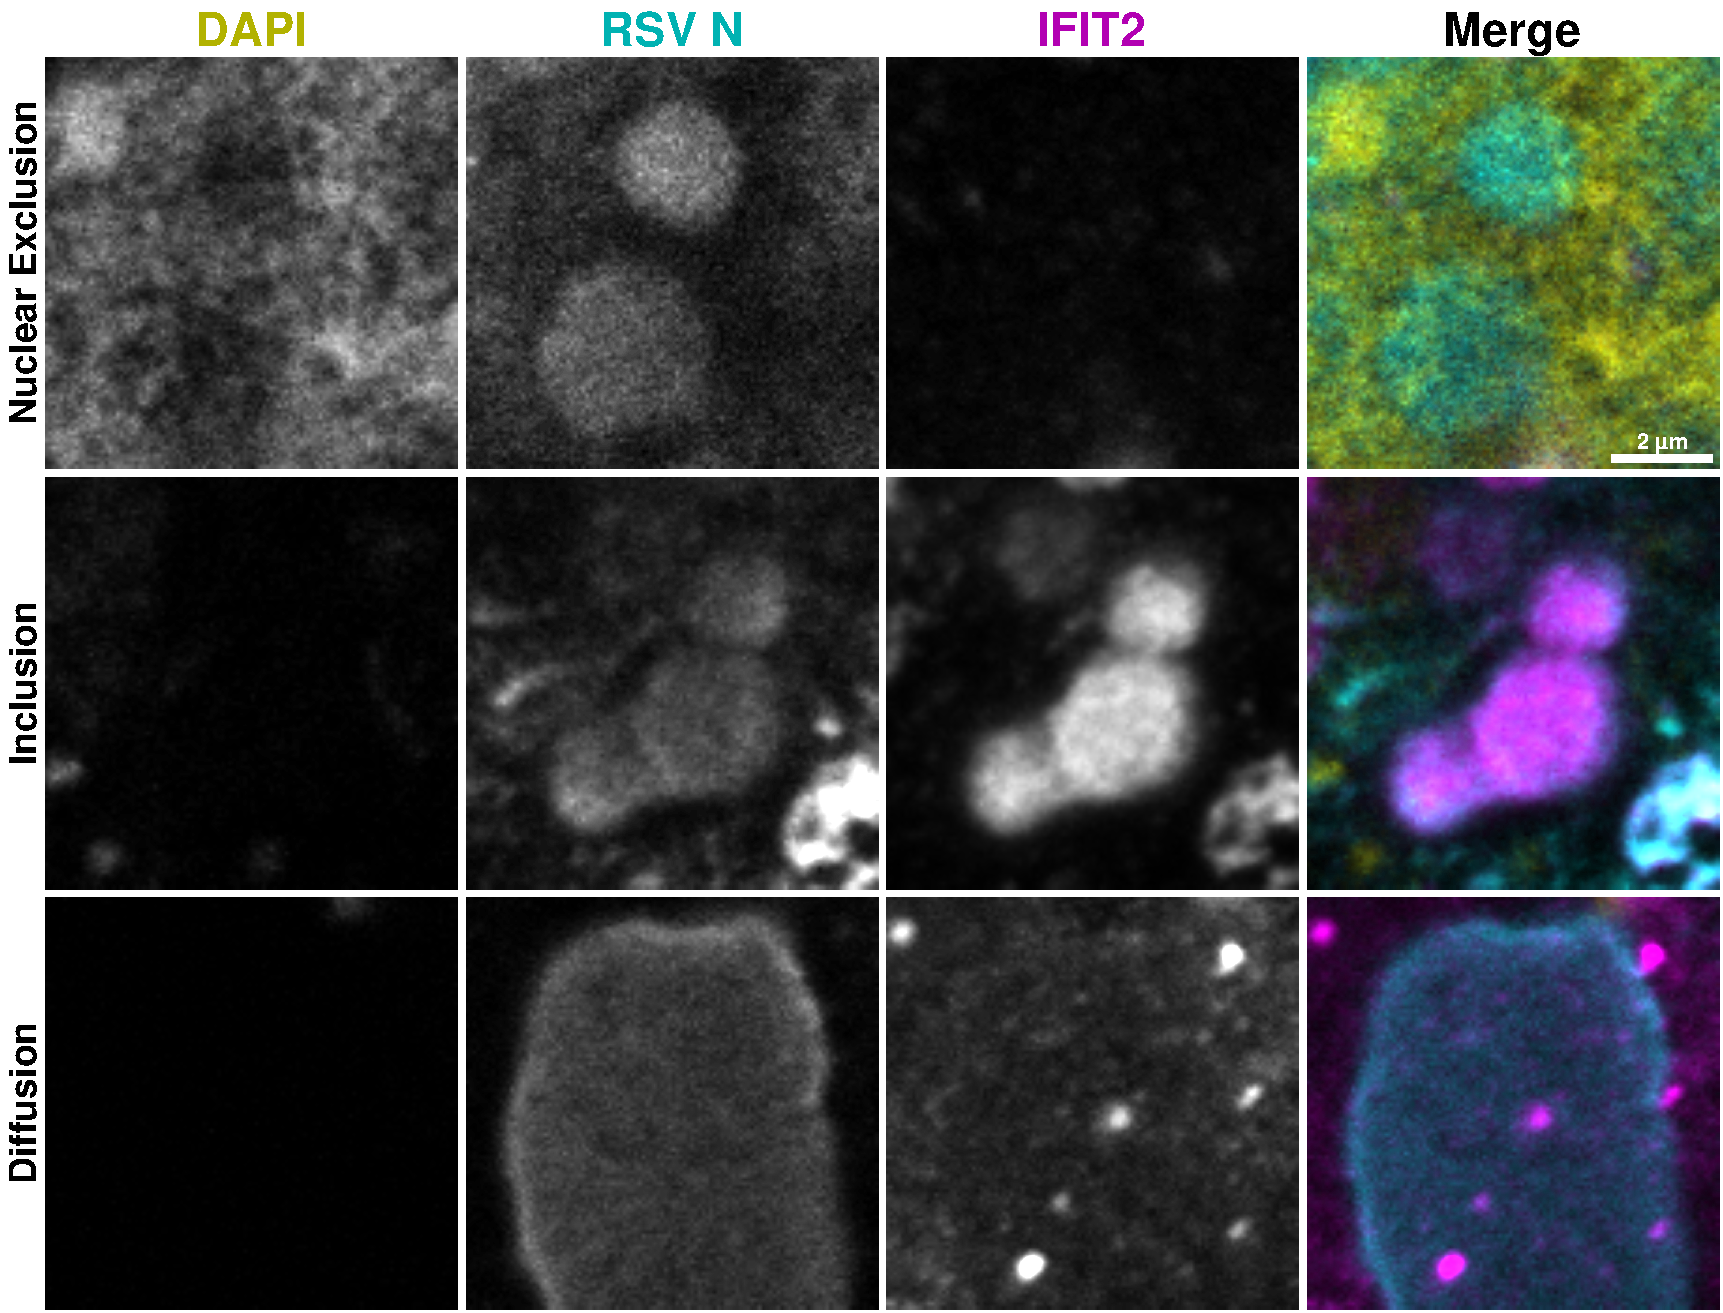
\includegraphics[width=1\linewidth]{08. Chapter 3/Figs/03. pIB/03. IFIT2/04. IFIT2-FLAG/03. FLAG/03. hi2f-hnhp.pdf}
    \caption[Representative Images of Observed Phenotypes of Exogenous Human IFIT2 in the Context of hRSV Pseudo Inclusion Bodies in VERO Cell Line, as Detected by FLAG Antibody.]{\textbf{Representative Images of Observed Phenotypes of Exogenous Human IFIT2 in the Context of hRSV Pseudo Inclusion Bodies in VERO Cell Line, as Detected by FLAG Antibody.} Vero cells were transfected with hRSV N and P, along with human IFIT2-FLAG containing plasmids using TransIT-X2 and were fixed after 24 hours. Cellular nuclei were stained with DAPI (yellow), and cells were double-labeled with anti-RSV N (cyan) and anti-FLAG (magenta) antibodies. This figure showcases representative examples of relevant phenotypes in the interaction between exogenous human IFIT2 and hRSV pseudo inclusion bodies. These phenotypes are presented in descending order based on their percentage proportions. The scale bar indicates 2 \(\mu \mbox{m}\).}
    \label{fig:Representative Images of Observed Phenotypes of Exogenous Human IFIT2 in the Context of hRSV Pseudo Inclusion Bodies in VERO Cell Line, as Detected by FLAG Antibody}
\end{figure}

49 35 21
0.23 2.1 0.7

Exogenous bovine IFIT2 colocalises with the edge of human pIB structures. This is unusual as human IFIT2 data suggest inclusions with regards to pIBs.  

\begin{figure}
    \begin{subfigure}{0.495\textwidth}
        \caption{}
        \includegraphics[width=1\linewidth]{08. Chapter 3/Figs/03. pIB/03. IFIT2/04. IFIT2-FLAG/03. FLAG/04. bar_bi2f_hnhp.pdf} 
    \end{subfigure}
    \begin{subfigure}{0.495\textwidth}
        \caption{}
        \includegraphics[width=1\linewidth]{08. Chapter 3/Figs/03. pIB/03. IFIT2/04. IFIT2-FLAG/03. FLAG/05. box_bi2f_hnhp.pdf}
    \end{subfigure}
    \caption[Observed Phenotypes of Exogenous Bovine IFIT2 in the Context of hRSV Pseudo Inclusion Bodies in VERO Cell Line, as Detected by FLAG Antibody.]{\textbf{Observed Phenotypes of Exogenous Bovine IFIT2 in the Context of hRSV Pseudo Inclusion Bodies in VERO Cell Line, as Detected by FLAG Antibody.} Vero cells were transfected with hRSV N and P, along with bovine IFIT2-FLAG containing plasmids using TransIT-X2 and were fixed after 24 hours. Cells were labeled with anti-RSV N and anti-FLAG antibodies and imaged on confocal microscope. Panel (a) shows percentual proportions of observed phenotypes between hRSV pseudo inclusion bodies and exogenous bovine IFIT2 (142 observations), with the red dotted line denoting the 5\% threshold, marking phenotypes considered relevant above this limit. Panel (b) shows the IB area in \(\mu \mbox{m}^2\) per observed relevant phenotype.}
    \label{fig:Observed Phenotypes of Exogenous Bovine IFIT2 in the Context of hRSV Pseudo Inclusion Bodies in VERO Cell Line, as Detected by FLAG Antibody}
\end{figure}

\begin{figure}
    \centering
    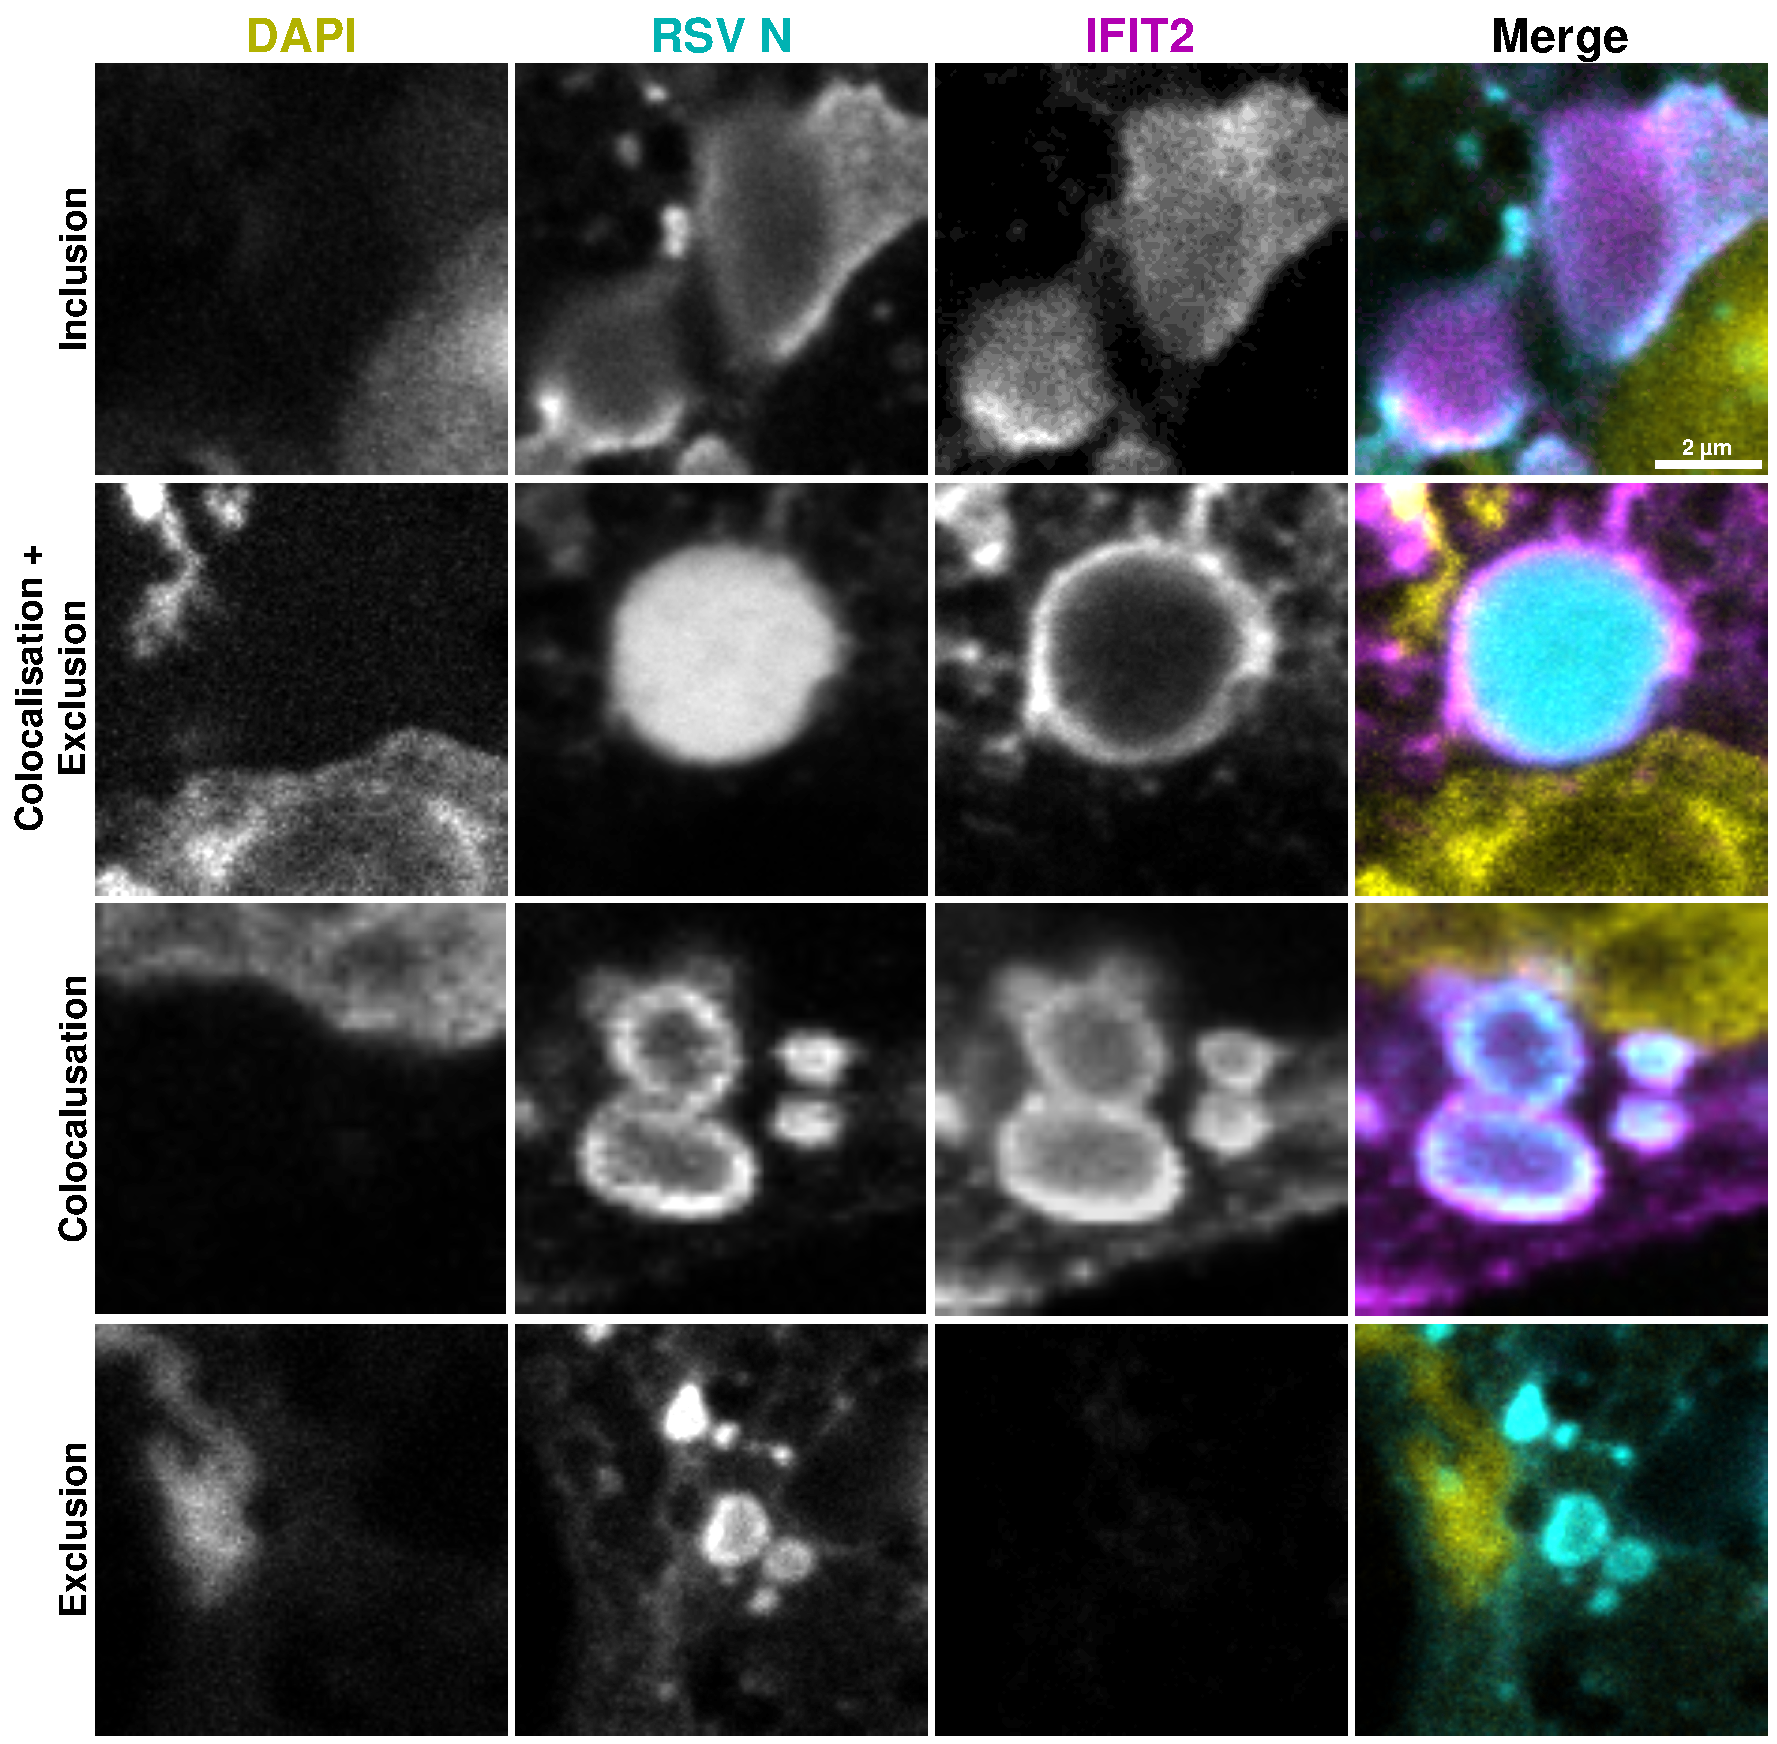
\includegraphics[width=1\linewidth]{08. Chapter 3/Figs/03. pIB/03. IFIT2/04. IFIT2-FLAG/03. FLAG/06. bi2f-hnhp.pdf}
    \caption[Representative Images of Observed Phenotypes of Exogenous Bovine IFIT2 in the Context of hRSV Pseudo Inclusion Bodies in VERO Cell Line, as Detected by FLAG Antibody.]{\textbf{Representative Images of Observed Phenotypes of Exogenous Bovine IFIT2 in the Context of hRSV Pseudo Inclusion Bodies in VERO Cell Line, as Detected by FLAG Antibody.} Vero cells were transfected with hRSV N and P, along with bovine IFIT2-FLAG containing plasmids using TransIT-X2 and were fixed after 24 hours. Cellular nuclei were stained with DAPI (yellow), and cells were double-labeled with anti-RSV N (cyan) and anti-FLAG (magenta) antibodies. This figure showcases representative examples of relevant phenotypes in the interaction between exogenous bovine IFIT2 and hRSV pseudo inclusion bodies. These phenotypes are presented in descending order based on their percentage proportions. The scale bar indicates 2 \(\mu \mbox{m}\).}
    \label{fig:Representative Images of Observed Phenotypes of Exogenous Bovine IFIT2 in the Context of hRSV Pseudo Inclusion Bodies in VERO Cell Line, as Detected by FLAG Antibody}
\end{figure}

46 31 12 6
1 2.8 2.8 1.7

\begin{figure}
    \begin{subfigure}{0.495\textwidth}
        \caption{}
        \includegraphics[width=1\linewidth]{08. Chapter 3/Figs/03. pIB/03. IFIT2/04. IFIT2-FLAG/03. FLAG/07. bar_bi2f_bnbp.pdf} 
    \end{subfigure}
    \begin{subfigure}{0.495\textwidth}
        \caption{}
        \includegraphics[width=1\linewidth]{08. Chapter 3/Figs/03. pIB/03. IFIT2/04. IFIT2-FLAG/03. FLAG/08. box_bi2f_bnbp.pdf}
    \end{subfigure}
    \caption[Observed Phenotypes of Exogenous Bovine IFIT2 in the Context of bRSV Pseudo Inclusion Bodies in VERO Cell Line, as Detected by FLAG Antibody.]{\textbf{Observed Phenotypes of Exogenous Bovine IFIT2 in the Context of bRSV Pseudo Inclusion Bodies in VERO Cell Line, as Detected by FLAG Antibody.} Vero cells were transfected with bRSV N and P, along with bovine IFIT2-FLAG containing plasmids using TransIT-X2 and were fixed after 24 hours. Cells were labeled with anti-RSV N and anti-FLAG antibodies and imaged on confocal microscope. Panel (a) shows percentual proportions of observed phenotypes between bRSV pseudo inclusion bodies and exogenous bovine IFIT2 (22 observations), with the red dotted line denoting the 5\% threshold, marking phenotypes considered relevant above this limit. Panel (b) shows the IB area in \(\mu \mbox{m}^2\) per observed relevant phenotype.}
    \label{fig:Observed Phenotypes of Exogenous Bovine IFIT2 in the Context of bRSV Pseudo Inclusion Bodies in VERO Cell Line, as Detected by FLAG Antibody}
\end{figure}

\begin{figure}
    \centering
    \includegraphics[width=1\linewidth]{08. Chapter 3/Figs/03. pIB/03. IFIT2/04. IFIT2-FLAG/03. FLAG/09. bi2f-bnbp.pdf}
    \caption[Representative Images of Observed Phenotypes of Exogenous Bovine IFIT2 in the Context of bRSV Pseudo Inclusion Bodies in VERO Cell Line, as Detected by FLAG Antibody.]{\textbf{Representative Images of Observed Phenotypes of Exogenous Bovine IFIT2 in the Context of bRSV Pseudo Inclusion Bodies in VERO Cell Line, as Detected by FLAG Antibody.} Vero cells were transfected with bRSV N and P, along with bovine IFIT2-FLAG containing plasmids using TransIT-X2 and were fixed after 24 hours. Cellular nuclei were stained with DAPI (yellow), and cells were double-labeled with anti-RSV N (cyan) and anti-FLAG (magenta) antibodies. This figure showcases representative examples of relevant phenotypes in the interaction between exogenous bovine IFIT2 and bRSV pseudo inclusion bodies. These phenotypes are presented in descending order based on their percentage proportions. The scale bar indicates 2 \(\mu \mbox{m}\).}
    \label{fig:Representative Images of Observed Phenotypes of Exogenous Bovine IFIT2 in the Context of bRSV Pseudo Inclusion Bodies in VERO Cell Line, as Detected by FLAG Antibody}
\end{figure}

100
0.41

\paragraph{The Impact of RNA-Binding on IFIT2-pIB Interaction}
%The Generation of Bovine IFIT2 RNA-Binding Mutant
Using published data about hIFIT2 rna-binding mutant

Difficulty of using alpha-fold with IFIT2 due to the swap domain

Using SWISS-MODEL to predict bIFIT2 structure from published hIFIT2 structures

Alignment of both structures, assessment of electrostatic charges and establishment of residues to be mutated

Primer design and mutagenesis procedure based on published hIFIT2 RNA-binding mutant paper
\cite{Tran2020InfluenzaMRNAs}

\begin{figure}
    \centering
    \includegraphics[width=1\linewidth]{08. Chapter 3/Figs/03. pIB/03. IFIT2/05. IFIT2-RNA binding mutant/01. Structure/01. structure.png}
    \caption[ifit2 mutant structure]{\textbf{bifit2 mutant structure.} redo this figure}
    \label{fig:ifit2 mutant structure}
\end{figure}


\begin{figure}
    \begin{subfigure}{0.495\textwidth}
        \caption{}
        \includegraphics[width=1\linewidth]{08. Chapter 3/Figs/03. pIB/03. IFIT2/05. IFIT2-RNA binding mutant/02. pIB/01. bar_bi2f24_hnhp.pdf} 
    \end{subfigure}
    \begin{subfigure}{0.495\textwidth}
        \caption{}
        \includegraphics[width=1\linewidth]{08. Chapter 3/Figs/03. pIB/03. IFIT2/05. IFIT2-RNA binding mutant/02. pIB/02. box_bi2f24_hnhp.pdf}
    \end{subfigure}
    \caption[Diverse Phenotypic Interactions of Bovine IFIT2 RNA-Binding Mutant with Human RSV Pseudo Inclusion Bodies (pIBs) in the VERO Cell Line.]{\textbf{Diverse Phenotypic Interactions of Bovine IFIT2 RNA-Binding Mutant with Human RSV Pseudo Inclusion Bodies (pIBs) in the VERO Cell Line.} Vero cells were transfected with hRSV N and P, along with bovine IFIT2-FLAG RNA-binding mutant containing plasmids using TransIT-X2 and were fixed after 24 hours. Cells were labeled with anti-RSV N and anti-FLAG antibodies and imaged on confocal microscope. Panel (a) shows percentual proportions of observed phenotypes between hRSV pseudo inclusion bodies and exogenous bovine IFIT2-FLAG RNA-binding mutant (548 observations), with the red dotted line denoting the 5\% threshold, marking phenotypes considered relevant above this limit. Panel (b) shows the IB area in \(\mu \mbox{m}^2\) per observed relevant phenotype.}
    \label{fig:Diverse Phenotypic Interactions of Bovine IFIT2 RNA-Binding Mutant with Human RSV Pseudo Inclusion Bodies (pIBs) in the VERO Cell Line}
\end{figure}

\begin{figure}
    \centering
    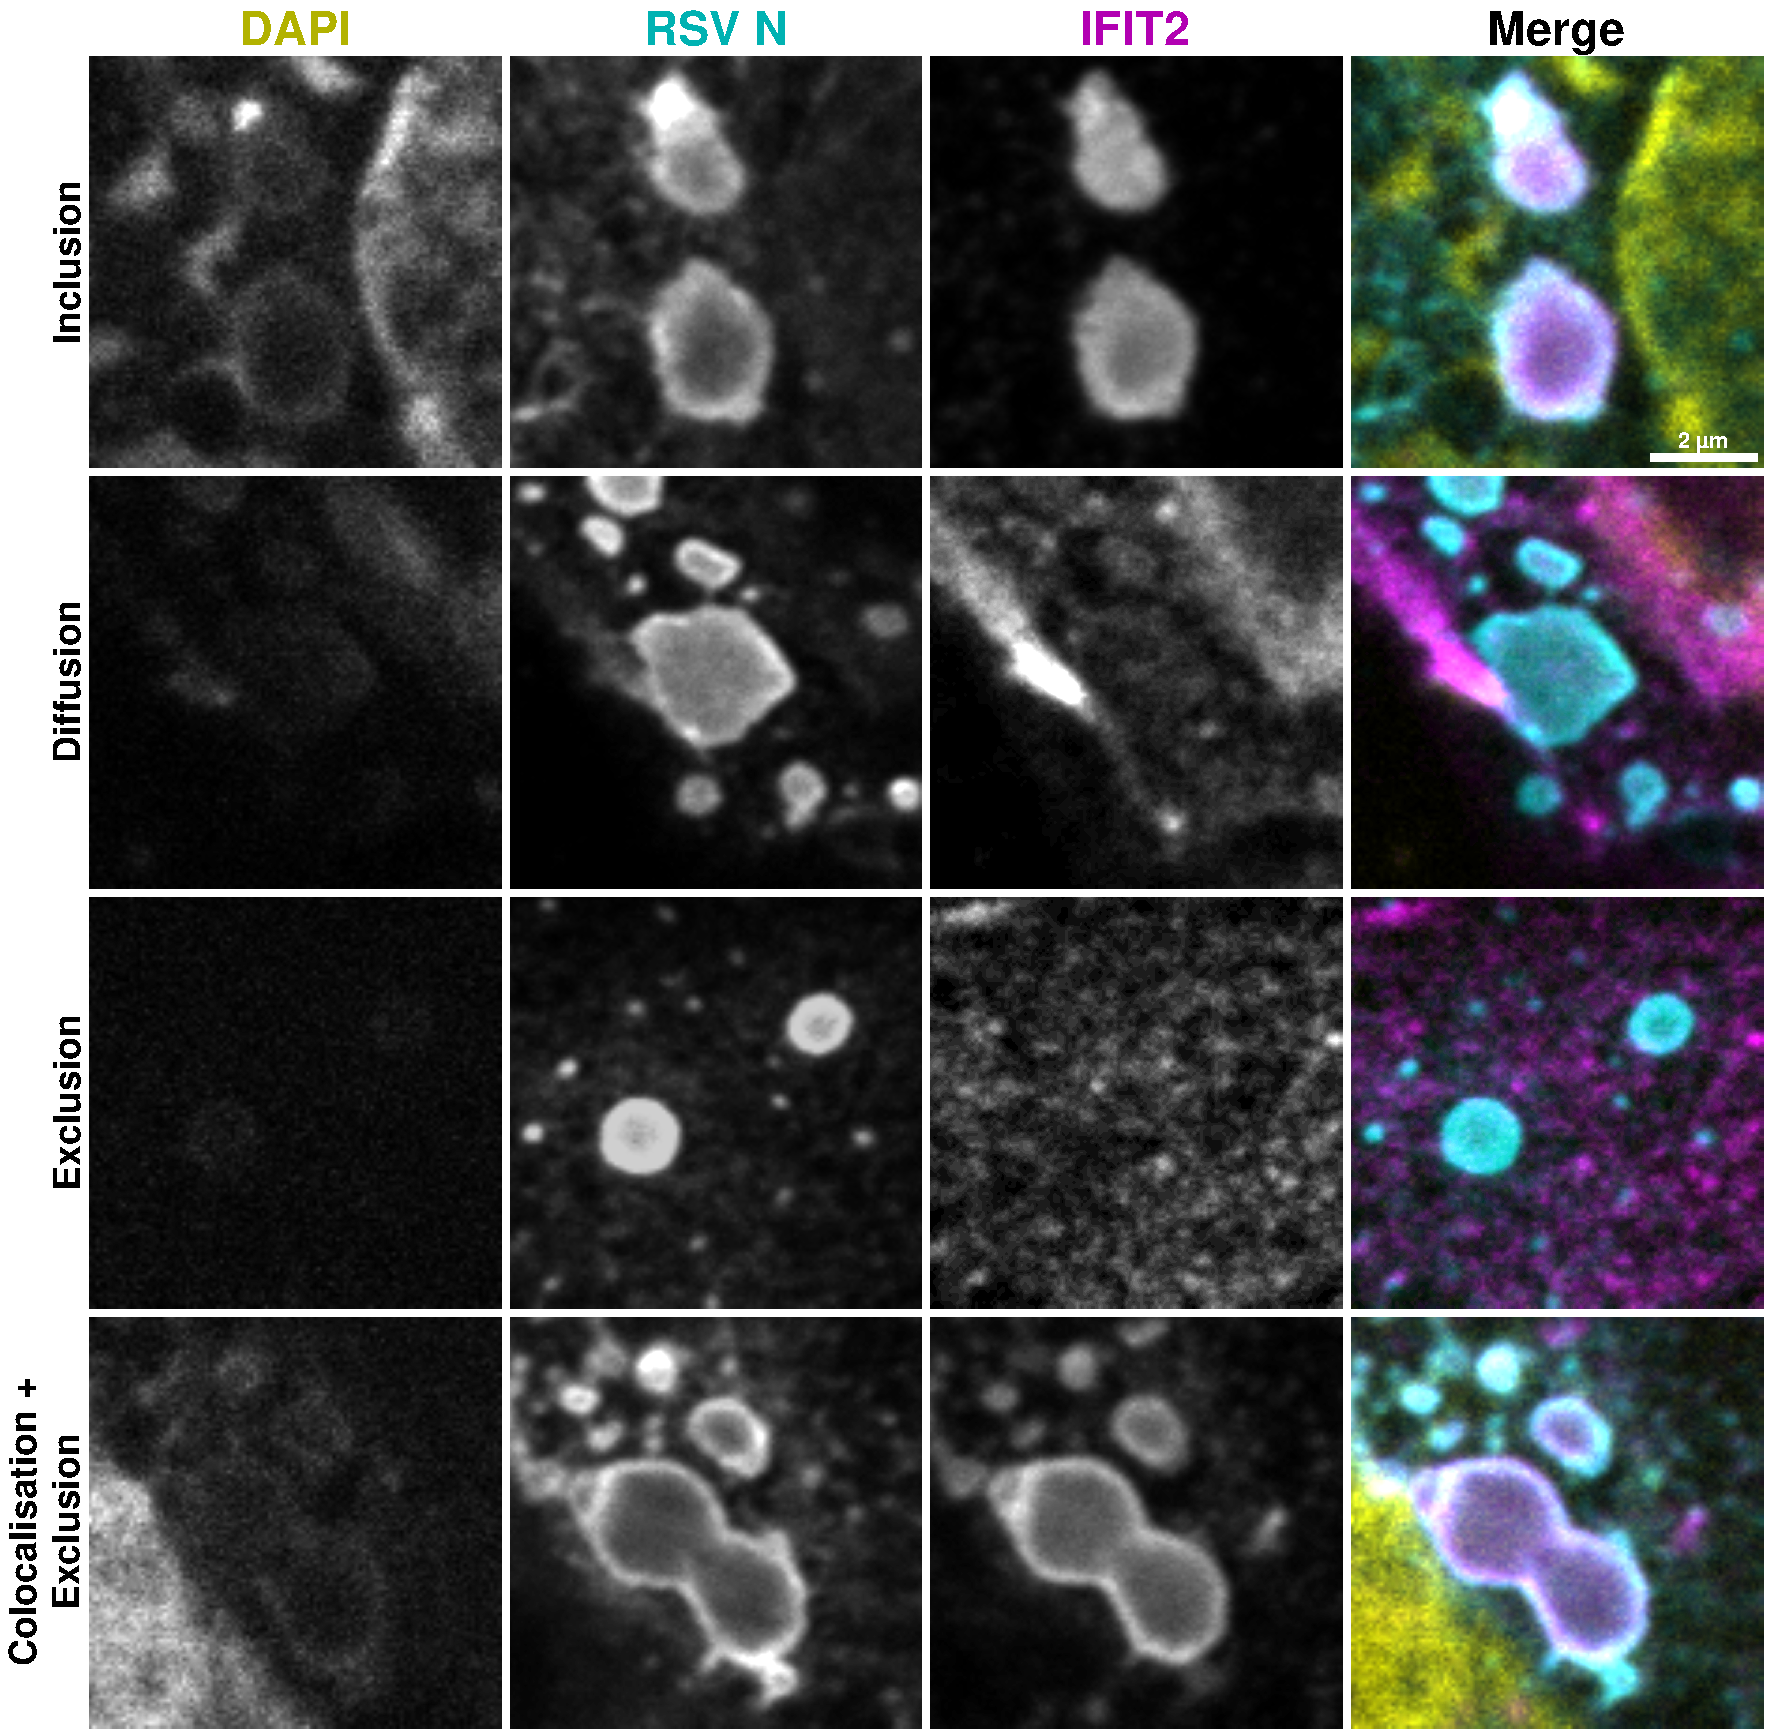
\includegraphics[width=1\linewidth]{08. Chapter 3/Figs/03. pIB/03. IFIT2/05. IFIT2-RNA binding mutant/02. pIB/03. bi2f24-hnhp.pdf}
    \caption[Representative Images of Diverse Phenotypic Interactions of Bovine IFIT2 RNA-Binding Mutant with Human RSV Pseudo Inclusion Bodies (pIBs) in the VERO Cell Line.]{\textbf{Representative Images of Diverse Phenotypic Interactions of Bovine IFIT2 RNA-Binding Mutant with Human RSV Pseudo Inclusion Bodies (pIBs) in the VERO Cell Line.}  Vero cells were transfected with bRSV N and P, along with bovine IFIT2-FLAG RNA-binding mutant containing plasmids using TransIT-X2 and were fixed after 24 hours. Cellular nuclei were stained with DAPI (yellow), and cells were double-labeled with anti-RSV N (cyan) and anti-FLAG (magenta) antibodies. This figure showcases representative examples of relevant phenotypes in the interaction between exogenous bovine IFIT2-FLAG RNA-binding mutant and hRSV pseudo inclusion bodies. These phenotypes are presented in descending order based on their percentage proportions. The scale bar indicates 2 \(\mu \mbox{m}\).}
    \label{fig:Representative Images of Diverse Phenotypic Interactions of Bovine IFIT2 RNA-Binding Mutant with Human RSV Pseudo Inclusion Bodies (pIBs) in the VERO Cell Line}
\end{figure}

49 27 13 11
0.8 0.5 1 1.8

\begin{figure}
    \begin{subfigure}{0.495\textwidth}
        \caption{}
        \includegraphics[width=1\linewidth]{08. Chapter 3/Figs/03. pIB/03. IFIT2/05. IFIT2-RNA binding mutant/02. pIB/04. bar_bi2f24_bnbp.pdf} 
    \end{subfigure}
    \begin{subfigure}{0.495\textwidth}
        \caption{}
        \includegraphics[width=1\linewidth]{08. Chapter 3/Figs/03. pIB/03. IFIT2/05. IFIT2-RNA binding mutant/02. pIB/05. box_bi2f24_bnbp.pdf}
    \end{subfigure}
    \caption[Diverse Phenotypic Interactions of Bovine IFIT2 RNA-Binding Mutant with Bovine RSV Pseudo Inclusion Bodies (pIBs) in the VERO Cell Line.]{\textbf{Diverse Phenotypic Interactions of Bovine IFIT2 RNA-Binding Mutant with Bovine RSV Pseudo Inclusion Bodies (pIBs) in the VERO Cell Line.} Vero cells were transfected with bRSV N and P, along with bovine IFIT2-FLAG RNA-binding mutant containing plasmids using TransIT-X2 and were fixed after 24 hours. Cells were labeled with anti-RSV N and anti-FLAG antibodies and imaged on confocal microscope. Panel (a) shows percentual proportions of observed phenotypes between bRSV pseudo inclusion bodies and exogenous bovine IFIT2-FLAG RNA-binding mutant (2 observations), with the red dotted line denoting the 5\% threshold, marking phenotypes considered relevant above this limit. Panel (b) shows the IB area in \(\mu \mbox{m}^2\) per observed relevant phenotype.}
    \label{fig:Diverse Phenotypic Interactions of Bovine IFIT2 RNA-Binding Mutant with Bovine RSV Pseudo Inclusion Bodies (pIBs) in the VERO Cell Line}
\end{figure}

\begin{figure}
    \centering
    \includegraphics[width=1\linewidth]{08. Chapter 3/Figs/03. pIB/03. IFIT2/05. IFIT2-RNA binding mutant/02. pIB/06. bi2f24-bnbp.pdf}
    \caption[Representative Images of Diverse Phenotypic Interactions of Bovine IFIT2 RNA-Binding Mutant with Bovine RSV Pseudo Inclusion Bodies (pIBs) in the VERO Cell Line.]{\textbf{Representative Images of Diverse Phenotypic Interactions of Bovine IFIT2 RNA-Binding Mutant with Bovine RSV Pseudo Inclusion Bodies (pIBs) in the VERO Cell Line.}  Vero cells were transfected with bRSV N and P, along with bovine IFIT2-FLAG RNA-binding mutant containing plasmids using TransIT-X2 and were fixed after 24 hours. Cellular nuclei were stained with DAPI (yellow), and cells were double-labeled with anti-RSV N (cyan) and anti-FLAG (magenta) antibodies. This figure showcases representative examples of relevant phenotypes in the interaction between exogenous bovine IFIT2-FLAG RNA-binding mutant and bRSV pseudo inclusion bodies. These phenotypes are presented in descending order based on their percentage proportions. The scale bar indicates 2 \(\mu \mbox{m}\).}
    \label{fig:Representative Images of Diverse Phenotypic Interactions of Bovine IFIT2 RNA-Binding Mutant with Bovine RSV Pseudo Inclusion Bodies (pIBs) in the VERO Cell Line}
\end{figure}

100
1.8

% summary i2
We have described how bovine IFIT2 RNA-binding mutant was designed based on the published human IFIT2 RNA-binding mutant data (needs to be annotated more). Overexpression of bovine IFIT2 RNA-binding mutant yields cellular distribution and morphology similar to what was observed with overexpressing human IFIT2-FLAG, suggesting that the mutant proteins are not toxic to the cells. In the first experiment where we were looking at interaction between bovine IFIT2 RNA-binding mutant and human pseudo inclusion bodies we saw several phenotypes. We observed bovine IFIT2 RNA-binding mutant being excluded from small and big pIBs and pIB associated filamentous network, while fully or partially colocalising with other pIBs. In a subsequent experiment we observed only colocalization and inclusion formation. When assessing the interaction between bovine IFIT2 RNA-binding mutant and human pIBs formed using wild-type human RSV P and GFP-tagged human RSV N, we observed consistently in two experiments that bovine IFIT2 RNA-binding mutant colocalises to the pIB structures.

\subsubsection{Nascent Moneky IFIT3 and Its Interaction With pIBs}
Nascent monkey IFIT3 seems to behave a if he pIB was not here. This means I has diffused phenotype. One exception is the top panel (shown with the arrow) which hints at concentrated IFIT3 at the edge of the pIBs. We do not know the localisation with respect to the pIB filaments as none were found in the slides. This data is as well supported by z stack measurements.

\begin{figure}
    \begin{subfigure}{0.495\textwidth}
        \caption{}
        \includegraphics[width=1\linewidth]{08. Chapter 3/Figs/03. pIB/04. IFIT3/01. bar_i3_vero.pdf} 
    \end{subfigure}
    \begin{subfigure}{0.495\textwidth}
        \caption{}
        \includegraphics[width=1\linewidth]{08. Chapter 3/Figs/03. pIB/04. IFIT3/02. box_i3_vero.pdf}
    \end{subfigure}
    \caption[Diverse Phenotypic Interactions of Monkey IFIT3 with Human Pseudo Inclusion Bodies (pIBs) in the VERO Cell Line.]{\textbf{Diverse Phenotypic Interactions of Monkey IFIT3 with Human Pseudo Inclusion Bodies (pIBs) in the VERO Cell Line.} Vero cells were transfected with hRSV N and P containing plasmids using TransIT-X2 and were fixed after 24 hours. Cells were labeled with anti-RSV N and anti-IFIT3 antibodies and imaged on confocal microscope. Panel (a) shows percentual proportions of observed phenotypes between hRSV pseudo inclusion bodies and monkey IFIT3 (39 observations), with the red dotted line denoting the 5\% threshold, marking phenotypes considered relevant above this limit. Panel (b) shows the IB area in \(\mu \mbox{m}^2\) per observed relevant phenotype.}
    \label{fig:Diverse Phenotypic Interactions of Monkey IFIT3 with Human Pseudo Inclusion Bodies (pIBs) in the VERO Cell Line}
\end{figure}

\begin{figure}
    \centering
    \includegraphics[width=1\linewidth]{08. Chapter 3/Figs/03. pIB/04. IFIT3/03. i3-vero-hnhp.pdf}
    \caption[Representative Images of Diverse Phenotypic Interactions of Monkey IFIT3 with Human Pseudo Inclusion Bodies (pIBs) in the VERO Cell Line.]{\textbf{Representative Images of Diverse Phenotypic Interactions of Monkey IFIT3 with Human Pseudo Inclusion Bodies (pIBs) in the VERO Cell Line.} Vero cells were transfected with hRSV N and P containing plasmids using TransIT-X2 and were fixed after 24 hours. Cellular nuclei were stained with DAPI (yellow), and cells were double-labeled with anti-RSV N (cyan) and anti-IFIT3 (magenta) antibodies. This figure showcases representative examples of relevant phenotypes in the interaction between monkey IFIT3 and hRSV pseudo inclusion bodies. These phenotypes are presented in descending order based on their percentage proportions. The scale bar indicates 2 \(\mu \mbox{m}\).}
    \label{fig:Representative Images of Diverse Phenotypic Interactions of Monkey IFIT3 with Human Pseudo Inclusion Bodies (pIBs) in the VERO Cell Line}
\end{figure}

41 36 15 5

4 2 4 3

\subsubsection{Nascent Moneky IFIT5 and Its Interaction With pIBs}
Nascent monkey IFIT5 colocalises with hRSV pseudo inclusion bodies (basically resembling the P staining). It also colocalises with pIB filamentous network. This network is only seen in cells that are co-transfected with RSV N and P proteins. We believe that they are an aftermath of a pIB breakdown. This data is as well supported by z stack measurements.

\begin{figure}
    \begin{subfigure}{0.495\textwidth}
        \caption{}
        \includegraphics[width=1\linewidth]{08. Chapter 3/Figs/03. pIB/05. IFIT5/01. bar_i5_vero.pdf} 
    \end{subfigure}
    \begin{subfigure}{0.495\textwidth}
        \caption{}
        \includegraphics[width=1\linewidth]{08. Chapter 3/Figs/03. pIB/05. IFIT5/02. box_i5_vero.pdf}
    \end{subfigure}
    \caption[Diverse Phenotypic Interactions of Monkey IFIT5 with Human Pseudo Inclusion Bodies (pIBs) in the VERO Cell Line.]{\textbf{Diverse Phenotypic Interactions of Monkey IFIT5 with Human Pseudo Inclusion Bodies (pIBs) in the VERO Cell Line.} Vero cells were transfected with hRSV N and P containing plasmids using TransIT-X2 and were fixed after 24 hours. Cells were labeled with anti-RSV N and anti-IFIT5 antibodies and imaged on confocal microscope. Panel (a) shows percentual proportions of observed phenotypes between hRSV pseudo inclusion bodies and monkey IFIT5 (100 observations), with the red dotted line denoting the 5\% threshold, marking phenotypes considered relevant above this limit. Panel (b) shows the IB area in \(\mu \mbox{m}^2\) per observed relevant phenotype.}
    \label{fig:Diverse Phenotypic Interactions of Monkey IFIT5 with Human Pseudo Inclusion Bodies (pIBs) in the VERO Cell Line}
\end{figure}

\begin{figure}
    \centering
    \includegraphics[width=1\linewidth]{08. Chapter 3/Figs/03. pIB/05. IFIT5/03. i5-vero-hnhp.pdf}
    \caption[Representative Images of Diverse Phenotypic Interactions of Monkey IFIT5 with Human Pseudo Inclusion Bodies (pIBs) in the VERO Cell Line.]{\textbf{Representative Images of Diverse Phenotypic Interactions of Monkey IFIT5 with Human Pseudo Inclusion Bodies (pIBs) in the VERO Cell Line.} Vero cells were transfected with hRSV N and P containing plasmids using TransIT-X2 and were fixed after 24 hours. Cellular nuclei were stained with DAPI (yellow), and cells were double-labeled with anti-RSV N (cyan) and anti-IFIT5 (magenta) antibodies. This figure showcases representative examples of relevant phenotypes in the interaction between monkey IFIT5 and hRSV pseudo inclusion bodies. These phenotypes are presented in descending order based on their percentage proportions. The scale bar indicates 2 \(\mu \mbox{m}\).}
    \label{fig:Representative Images of Diverse Phenotypic Interactions of Monkey IFIT5 with Human Pseudo Inclusion Bodies (pIBs) in the VERO Cell Line}
\end{figure}

62 38

1.2 4

% summary
Endogenous human IFIT1 seems to be diffused through the human pIB structure. On the other hand, endogenous monkey IFIT1 forms an inclusion in human pIBs, colocalises with the edge of human and bovine pIBs and is excluded from the filamentous pIB network. This suggests that the colocalization is not caused by mere interaction with N or P but its dependant on the integrity of pIBs.

Endogenous monkey IFIT3 seems to be diffuse through the human pIB structures (with maybe a small hint of colocalization).

Endogenous monkey IFIT5 colocalises with human pIBs and with the NP network (this network is never present in infected cells, so we do not know how are other IFIT5s colocalising with it).